% PEX_KERNEL_REVISION_MAIN
\documentclass[conference,9pt,letterpaper]{IEEEtran}
\usepackage[T1]{fontenc}
\usepackage{amsmath,amssymb,graphicx,booktabs,array,microtype}
\usepackage[hidelinks]{hyperref}
\usepackage[ruled,vlined,linesnumbered]{algorithm2e}
\SetKwInOut{Input}{Input}
\SetKwInOut{Output}{Output}
\DontPrintSemicolon
\SetAlFnt{\scriptsize}
\SetAlCapFnt{\footnotesize}
\SetAlCapNameFnt{\footnotesize}
\SetAlgoNlRelativeSize{-1}

\hypersetup{pdfauthor={},pdftitle={Learning to Populate Capacitance Evaluation Tables for Rule-Based Parasitic Extraction}}
\newcommand{\nrmse}{\operatorname{NRMSE}}
\title{Learning to Populate Capacitance Evaluation Tables for Rule-Based Parasitic Extraction}
\author{\IEEEauthorblockN{Anonymous authors}\IEEEauthorblockA{\vphantom{Department and affiliation}\vphantom{City, Country}\\\vphantom{Contact information}}}
\begin{document}
\bstctlcite{dac:bibcontrol}
\maketitle
\begin{abstract}
Rule-based parasitic extraction must evaluate geometries absent from a finite characterization set. We propose Full, an observation-conditioned residual model that combines a numerical anchor, Transformer residuals, and applicable numerical corrections through component-wise gating. Predictions populate eligible native compute-table entries during preparation, preserving supplied observations, resistance, runtime lookup, and parasitic-network assembly. Across public rules, finite-element data, and cross-process transfer, Full lowers condition-level macro normalized root-mean-square error (NRMSE) relative to the OpenRCX kernel and multilinear interpolation with sparse-support extension in all 60 evaluated conditions spanning 10--70\% characterization holdout; Binary and Ungated do so in 55 and 50 conditions. This empirical consistency motivates Full as the default, without implying optimality on every condition or downstream metric. Separate fixed-node rule-export experiments improve capacitance and worst-slack fidelity in all 16 layout--budget settings. A new four-arm sparse-native comparison completes 48 paired settings with hidden observations removed before native table construction: Full improves net-capacitance and worst-slack fidelity over Native-sparse in 7/16 and 9/16 seed-averaged cells. Thus the offline consistency does not imply universal downstream gains. The distinct full-characterization compute-table path keeps mean extraction time within 3.6\% of native extraction, with recorded external preparation stages totaling 5.41--13.99\,s.
\end{abstract}

\section{Introduction}
Parasitic extraction supplies electrical models for static
timing analysis (STA). Rule-based extractors query precharacterized capacitance tables as widths, spacings, and neighboring layers vary across a routed design.
Rule-based parasitic extraction separates process characterization from layout evaluation. Reference capacitances for representative interconnect geometries are encoded in empirical models or lookup tables, and layout extraction evaluates the corresponding models for encountered structures~\cite{tsai,yang2023cnncap}. OpenRCX provides a concrete example: its extraction rules are calibrated from reference parasitics and are evaluated using coupling distance and surrounding routing context~\cite{orcx_runtime,openrcx}.

A finite set of characterization points does not coincide with every geometric configuration encountered in a routed layout. Between sampled points, the extractor must estimate capacitance using the available rule data. Model-library accuracy therefore depends not only on pattern coverage but also on how the nonlinear geometry--capacitance response is represented between characterization points~\cite{zhou2026rmlpcap}. Increasing characterization density can improve that representation, but also increases the amount of reference data that must be generated and stored~\cite{yang2023cnncap}. This motivates improving rule evaluation while holding the available characterization samples fixed.

Prior work has automated pattern and formula construction from field-solver samples~\cite{li2020autoprechar}, developed neural capacitance and matrix predictors~\cite{yang2023cnncap,zhou2026rmlpcap,attentioncap,flash}, and studied geometry and layer-thickness exploration~\cite{tsai}. We focus on the complementary problem of estimating uncharacterized queries from a supplied set of process-specific characterization samples.

\begin{figure}[t]
\centering\includegraphics[width=\columnwidth]{dac_layout_query_revision/figures/Schematic diagram of the rule-driven parasitic parameter extraction process.png}
\caption{Schematic diagram of the rule-driven parasitic parameter extraction process.}
\label{fig:OpenRCX}
\end{figure}

We propose Full, which conditions a numerical anchor and Transformer residual on supplied capacitance samples, geometry, and material context. Component-wise gating fuses applicable numerical and neural corrections. Parameters remain fixed during conditional inference, while observations alter predictions. Predicted rule values can be exported into the native flow.
A target table supplies candidate geometries, structural/material context, and observed geometry–capacitance pairs. These observations reveal its local electrical response and complement information learned from other tables. Conditioning on them updates the completed table while keeping learned parameters fixed, even when the target has too few observations to train a flexible model independently.

Our predictor learns residual corrections to an anchor constructed from the available support. Geometry tokens bind positions to observation indicators, known capacitances, and anchor values; material tokens supply context. A shared Transformer associates queries with the observed response. Full uses component-wise gating to combine the applicable numerical and neural corrections. It preserves characterized entries and supplies predicted capacitances to the native extraction flow.

The deployment interface matters as much as prediction cost. Direct neural evaluation is slower than a native lookup. We therefore prepare learned values in the internal compute table, retaining the original getter and downstream RC assembly.
% This interface differs from exporting predictions at existing characterization-file nodes. Both configurations are evaluated and named separately.
We evaluate controlled characterization subsampling, support-size sensitivity, cross-process prediction, and native extraction fidelity.
%dense, smooth supports may already favor simple interpolation.
Full achieves lower error than the OpenRCX kernel and the extended MLI baseline in all 60 evaluated characterization-holdout conditions. We retain Full as the unified default for the consistency of these improvements across the evaluated domains and support conditions. Ungated and Binary improve over both baselines in 50 and 55 conditions, respectively; they can nevertheless have lower error than Full locally. This is a post-hoc empirical choice, not a guarantee for arbitrary unseen applications.

Full improves over the Binary ablation in all five finite-element (FEM) coverage conditions at 30\% missingness. At fixed sparse budgets, a target-adapted MLP is more accurate on several FEM and transfer conditions. Full improves rule-export net-capacitance
and worst-slack fidelity over MLI-ext. in all 16 layout–budget conditions, while Binary has lower timing-tail error in ten. We therefore evaluate coverage, observation count, and downstream use together.


The contributions are (i) Full, a characterization-conditioned predictor with gated fusion of numerical and learned residuals; (ii) a finite-distance compute-table population interface that preserves measurement entries, resistance and native query assembly; and (iii) matched production-kernel comparisons connecting coverage sensitivity, measured layout queries, independent template references and extraction costs.
%The evaluation retains conditions where numerical or simpler learned methods are better.

\section{Problem and Related Work}
\subsection{Rule-based capacitance evaluation}
A rule is identified by process/corner, pattern family and layer context. Characterization supplies geometry--capacitance samples. A preparation stage builds internal lookup structures, after which extraction maps a layout request to a pattern/width and evaluates the corresponding distance response. Native quantization and boundary behavior are part of this algorithm.
%equality of a floating-point interpolation formula does not imply equality of the complete evaluator.

\subsection{Measured off-grid demand}
Across two instrumented OpenRCX getters on eight unchanged routed layouts, we record 9,888,586 calls and 19,562 unique rule/geometry keys. The calls comprise 2,696,515 node hits, 4,547,424 non-node requests inside the selected width slice, 967,755 outside it, and 1,676,892 fringe/special requests. Raw non-node requests account for 55.77\% of all logged calls and 67.16\% of finite-distance calls (Fig.~\ref{fig:census}). Native width mapping and compute-grid quantization send 849,663 raw non-node requests to effective characterization nodes. Ordered trace alignment matches geometry and original returned capacitances for all 8,211,694 finite getter calls. Full-support population changes 924,647 returns: 11.26\% of finite calls and 9.35\% of all logged calls. These are numerical changes, not measured improvements against physical truth. The raw non-node, mapped-node, and populated sets are not interchangeable.

\begin{figure}[t]
\centering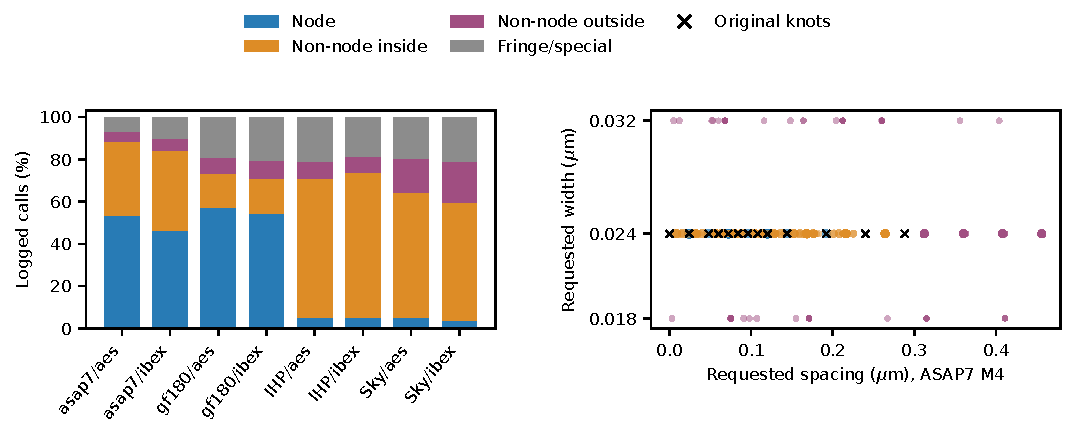
\includegraphics[width=\columnwidth]{figures/query_census.pdf}
\caption{Measured non-node demand. Left: occurrence-weighted query classes over two logged capacitance getters on eight fixed layouts. Right: ASAP7 M4 requests and original knots; marker area reflects log occurrence.
%Counts exclude resistance, five-argument diagonal getters and later assembly; they are neither capacitance nor runtime weights. Raw and effective node identities differ under native mapping.
}
\label{fig:census}
\end{figure}
The trace preserves SPEF electrical records on all layouts.

% It establishes the frequency of non-node evaluation in these getters, not the fraction of all PEX work. Characterization holdout is a different quantity: it varies the available information rather than measuring runtime request frequency. We evaluate all four requested holdout levels without equating them to the census percentages.

\subsection{Problem formulation and kernel scope}
For context $c$, available observations $S=\{(x_i,y_i)\}$ and query coordinates $Q$, the estimator satisfies
\begin{equation}
\widehat y_Q=F_\theta(S,Q,c),\qquad \widehat y(x_i)=y_i\ (x_i\in S).
\end{equation}
An off-grid geometry need not lie outside support. Inside-support classification requires affine-space and hull membership;
% incompatible topologies or outputs are excluded explicitly.
Only S values enter prediction; query reference values enter scoring.

Commercial sign-off parasitic extraction tools, including
Siemens Calibre xACT \cite{siemens_calibre_xact}, Calibre xACT 3D \cite{siemens_calibre_xact3d}, and Synopsys StarRC \cite{synopsys_starrc},
are not considered direct algorithmic baselines in this work, as these tools are integrated extraction platforms that incorporate or provide access to field-solver-based extraction capabilities, rather than standalone implementations of pattern-matching-based lookup-table interpolation.
Our controlled algorithmic comparison uses OpenRCX \cite{openroad_openrcx} and a specified generic numerical interpolation baseline with identical observable support. Commercial product-level comparisons would require matched characterization inputs and access to equivalent evaluation interfaces.

The primary algorithmic comparison is the pinned OpenRCX finite-distance kernel and specified multilinear interpolation (MLI). MLI is a generic tensor interpolation baseline; we do not establish equivalence to a proprietary Calibre xRC kernel. %This comparison concerns the interpolation operator,
%commercial binaries and product-specific boundary policies are outside its scope.
Complete cells require $2^d$ vertices, in $d$ dimensions,
\begin{equation}
\widehat y(x)=\sum_{\epsilon\in\{0,1\}^d}y_\epsilon
 \prod_{j=1}^d t_j^{\epsilon_j}(1-t_j)^{1-\epsilon_j}.
\end{equation}
% Sparse-support completion and boundary clamping are separately declared extensions, not attributed to xRC.
Physical data have rank one or two; four-dimensional evaluation is an implementation test only. OpenRCX comparison retains native width selection, integer geometry and four-unit compute bins; a continuous-distance variant isolates quantization effects. General numerical predictors are component controls.
For two-dimensional FEM/transfer inputs, the first coordinate selects a
characterized width slice using the native width map, and the second is
separation within that slice. Micrometer coordinates are rounded to integer
units at scale 1,000 for these kernel comparisons; distance indices use
four-unit bins. Single-point and boundary slices return their characterized
endpoint values. Each capacitance component uses this same scalar operator;
this adaptation does not reproduce an arbitrary multidimensional extractor.

\subsection{Related models and interfaces}
AttentionCap predicts capacitance matrices from conductor/material tokens~\cite{attentioncap}; Flash-CNNCap predicts window contributions in a three-dimensional DEF-to-SPEF workflow~\cite{flash}.
AttentionCap itself supports partial matrix-row supervision. Our component-supervised AttentionCap adaptation tests a specified observation budget and fitting recipe.
% rather than a general limit of matrix architectures.
Flash-CNNCap's 3D window task is not converted into a mismatched 2D speed ranking.
ResCap corrects initial physical estimates~\cite{rescap}; hybrid PEX selects extraction methods by window~\cite{hybrid}. Here the anchor uses current observations and fusion acts within a rule. CNPs~\cite{cnp} and attentive neural processes~\cite{anp} provide conditional regression interfaces, and is evaluated as such.
%not categorized as a field solver.

% \section{Estimator and Compute-Table Preparation}
% % \subsection{Observation-conditioned residual fusion}
% % The anchor uses piecewise-linear interpolation for rank-one support, simplex interpolation inside higher-rank support, and nearest-observation fallback outside or for degeneracy. Tokens encode geometry, context/materials, observation status, observed values and the anchor. Source-fitted scaling remains fixed. The observation indicator distinguishes an unobserved placeholder from an observed zero.

% % With representation $h_i$, anchor $b_{i,k}$ and correction candidates $\Delta_{i,e,k}$, predictions are
% % \begin{equation}
% % \widehat y_{i,k}=\left[b_{i,k}+\sum_{e\in\mathcal E_i}\pi_{i,e,k}\Delta_{i,e,k}\right]_+ .
% % \end{equation}
% % The gate reads the representation and support density, distance, span, hull membership and correction disagreement. Binary combines zero and raw neural correction. Ungated adds the raw neural correction directly. Full additionally uses applicable PCHIP, aligned-width interpolation, six RBF-GP configurations and an envelope-clipped neural correction. These candidates are existing algorithm components; all applicable branches execute before fusion. Affine/IDW controls are not retrospectively described as model ablations.

% % The encoder has two layers, four heads and width 64; the gate hidden width is 32. Matched Full/Binary/Ungated training uses the same source pools, residual initialization, optimizer, update counts and three seeds. AdamW uses learning rate $2\times10^{-4}$ and weight decay $10^{-4}$; a source-scaled Huber loss supervises withheld components. Training masks span random, block, boundary and eligible whole-width patterns at 10/30/50/70\% holdout. The query--query attention makes outputs batch-conditioned.


% %%%%%%%%%%%%%%%%%%%%%%%%%%%%%%%%%%%%%%%%%%%%%%%%%%%%
% \subsection{Observation-conditioned residual fusion}
% \label{subsec:residual_fusion}

% Given a characterization table, let
% $\mathcal{S}=\{(\mathbf{x}_j,\mathbf{y}_j)\}_{j=1}^{N}$
% denote the available observations, where $\mathbf{x}_j$
% represents the geometry and process-related context, and
% $\mathbf{y}_j\in\mathbb{R}^{K}$ contains the corresponding
% capacitance components. For a set of query geometries
% $\mathcal{Q}=\{\mathbf{x}_i\}_{i=1}^{M}$, the objective is to
% estimate their capacitances without accessing their reference
% values during inference. We construct an observation-conditioned
% estimator that combines a numerical interpolation anchor with
% multiple candidate residual corrections through a learned
% component-wise gating mechanism.

% \textbf{Input encoding and contextual representation.}
% For each observation and query, the input representation
% encodes its geometry, process and layer context, observation
% status, available capacitance values, and numerical anchor.
% In particular, an observation indicator distinguishes an
% unobserved entry from an observed zero-valued capacitance.
% The resulting token features are mapped into a
% $d$-dimensional embedding:
% \begin{equation}
% \mathbf{z}_i^{(0)}
% =
% \mathbf{W}_{\mathrm{in}}\mathbf{x}_i^{\mathrm{feat}}
% +
% \mathbf{b}_{\mathrm{in}},
% \label{eq:input_embedding}
% \end{equation}
% where $\mathbf{x}_i^{\mathrm{feat}}$ denotes the encoded
% feature vector and $d=64$ is the hidden dimension.
% The embedded observation and query tokens are processed
% jointly by a Transformer encoder with two layers and four
% attention heads:
% \begin{equation}
% \mathbf{H}^{(L)}
% =
% \operatorname{TransformerEncoder}
% \left(\mathbf{Z}^{(0)}\right),
% \qquad L=2.
% \label{eq:transformer_encoder}
% \end{equation}
% The contextual representation of query $i$ is
% \begin{equation}
% \mathbf{h}_i
% =
% \mathbf{H}^{(L)}_i
% \in\mathbb{R}^{d}.
% \label{eq:query_representation}
% \end{equation}
% The attention mask excludes padded tokens, while the joint
% encoding allows each query representation to incorporate
% the available characterization context.

% \textbf{Numerical anchor and residual generation.}
% We first construct a numerical anchor $b_{i,k}$ for each
% query $i$ and capacitance component $k$. Piecewise-linear
% interpolation is used for rank-one support, simplex
% interpolation for higher-rank support, and nearest-observation
% fallback for extrapolation or degenerate configurations.
% The anchor provides a numerical reference that preserves
% the information contained in the available characterization
% samples.

% A neural residual head predicts a data-driven correction
% from the contextual representation:
% \begin{equation}
% \Delta_{i,\mathrm{NN},k}
% =
% \mathbf{w}_{k}^{\mathsf T}\mathbf{h}_i
% +
% b_k^{\mathrm{NN}},
% \label{eq:neural_residual}
% \end{equation}
% where $\mathbf{w}_k$ and $b_k^{\mathrm{NN}}$ are learnable
% parameters. To constrain the neural prediction within the
% observation-supported envelope, we additionally construct
% a clipped residual:
% \begin{equation}
% \Delta_{i,\mathrm{clip},k}
% =
% \operatorname{clip}
% \left(
% b_{i,k}+\Delta_{i,\mathrm{NN},k},
% L_{i,k},U_{i,k}
% \right)-b_{i,k},
% \label{eq:clipped_residual}
% \end{equation}
% where $L_{i,k}$ and $U_{i,k}$ denote the lower and upper
% bounds of the support-derived envelope. This constraint is
% applied to queries inside the characterized support;
% outside it, the unconstrained neural residual is retained.

% In addition to the two neural corrections, we construct
% a dictionary of applicable classical numerical corrections,
% including the selected interpolation and regression-based
% candidates. Let $\mathcal{E}_i$ denote the complete candidate
% set for query $i$. Each candidate provides a residual
% correction relative to the common anchor:
% \begin{equation}
% \Delta_{i,e,k}
% =
% f_{i,e,k}-b_{i,k},
% \qquad e\in\mathcal{E}_i,
% \label{eq:correction_definition}
% \end{equation}
% where $f_{i,e,k}$ is the candidate prediction. The neural
% and clipped-neural residuals are appended to this dictionary.
% A binary applicability indicator $m_{i,e}$ identifies
% whether candidate $e$ is valid for query $i$.

% \textbf{Agreement-aware gating.}
% The contribution of each candidate is determined by a
% learned gate conditioned on both the query representation
% and the local characterization support. We first construct
% a support descriptor
% \begin{equation}
% \mathbf{u}_i
% =
% [
% \rho_i,\,
% d_i,\,
% s_i,\,
% q_i
% ],
% \label{eq:support_descriptor}
% \end{equation}
% where $\rho_i$ denotes support density, $d_i$ the distance
% to available observations, $s_i$ the support span, and
% $q_i$ the hull-membership indicator.

% To characterize the agreement among applicable correction
% candidates, we calculate their component-wise mean,
% standard deviation, and range:
% \begin{align}
% \mu_{i,k}
% &=
% \frac{\sum_{e\in\mathcal{E}_i}
% m_{i,e}\Delta_{i,e,k}}
% {\sum_{e\in\mathcal{E}_i}m_{i,e}},
% \\
% \sigma_{i,k}
% &=
% \sqrt{
% \frac{\sum_{e\in\mathcal{E}_i}
% m_{i,e}(\Delta_{i,e,k}-\mu_{i,k})^2}
% {\sum_{e\in\mathcal{E}_i}m_{i,e}}
% +\epsilon},
% \\
% r_{i,k}
% &=
% \max_{e:m_{i,e}=1}\Delta_{i,e,k}
% -
% \min_{e:m_{i,e}=1}\Delta_{i,e,k},
% \label{eq:agreement_statistics}
% \end{align}
% where $\epsilon$ is a small numerical constant.
% These statistics quantify the local disagreement among
% candidate corrections.

% The gate input is formed by concatenating the contextual
% representation, support descriptor, and agreement statistics:
% \begin{equation}
% \mathbf{v}_i
% =
% [
% \mathbf{h}_i;
% \mathbf{u}_i;
% \boldsymbol{\mu}_i;
% \boldsymbol{\sigma}_i;
% \mathbf{r}_i
% ].
% \label{eq:gate_input}
% \end{equation}
% A two-layer multilayer perceptron produces component-wise
% candidate logits:
% \begin{equation}
% \mathbf{a}_i
% =
% \mathbf{W}_{g,2}
% \operatorname{ReLU}
% \left(
% \mathbf{W}_{g,1}\mathbf{v}_i
% +
% \mathbf{b}_{g,1}
% \right)
% +
% \mathbf{b}_{g,2},
% \label{eq:gate_logits}
% \end{equation}
% where the output is reshaped into
% $\mathbf{a}_i\in\mathbb{R}^{|\mathcal{E}_i|\times K}$.
% The hidden dimension of the gating network is 32.

% The candidate weights are obtained through a masked
% component-wise softmax:
% \begin{equation}
% \pi_{i,e,k}
% =
% \frac{
% m_{i,e}
% \exp\left((a_{i,e,k}+\beta_e)/\tau\right)
% }{
% \sum_{j\in\mathcal{E}_i}
% m_{i,j}
% \exp\left((a_{i,j,k}+\beta_j)/\tau\right)
% },
% \label{eq:gating_weights}
% \end{equation}
% where $\beta_e$ is a learnable candidate-specific prior
% bias and $\tau>0$ is a learnable temperature. Invalid
% candidates are excluded from normalization. The anchor
% itself is represented by a zero residual correction and
% remains available for every query. The prior biases
% initialize the nonzero classical corrections with a
% negative logit offset, while the neural correction branches
% and anchor start without such suppression.

% \textbf{Residual fusion and physical projection.}
% Finally, the estimator combines the numerical anchor with
% the weighted candidate corrections:
% \begin{equation}
% \widetilde{y}_{i,k}
% =
% b_{i,k}
% +
% \sum_{e\in\mathcal{E}_i}
% \pi_{i,e,k}\Delta_{i,e,k}.
% \label{eq:residual_fusion}
% \end{equation}
% Since capacitance values must be non-negative, the final
% prediction is projected onto the non-negative domain:
% \begin{equation}
% \boxed{
% \widehat{y}_{i,k}
% =
% \max(0,\widetilde{y}_{i,k})
% =
% \left[
% b_{i,k}
% +
% \sum_{e\in\mathcal{E}_i}
% \pi_{i,e,k}\Delta_{i,e,k}
% \right]_+
% }.
% \label{eq:final_prediction}
% \end{equation}
% Here, $[\cdot]_+$ denotes element-wise non-negative
% projection. The component-wise gating mechanism allows
% different capacitance components to select different
% correction mixtures according to their local support
% conditions and candidate agreement.

% All source-fitted feature scaling parameters remain fixed
% during inference. The model is trained using masked
% characterization episodes, where observed entries form the
% input support and withheld entries provide supervision.
% The final predictions are optimized using a source-scaled
% Huber objective:
% \begin{equation}
% \mathcal{L}_{\mathrm{Huber}}
% =
% \frac{1}{|\mathcal{Q}|K}
% \sum_{i\in\mathcal{Q}}
% \sum_{k=1}^{K}
% \operatorname{Huber}_{\delta}
% \left(
% \frac{\widehat{y}_{i,k}-y_{i,k}}{s_k}
% \right),
% \label{eq:training_loss}
% \end{equation}
% where $y_{i,k}$ is the withheld reference capacitance,
% $s_k$ is the source-derived scale for component $k$, and
% $\delta$ is the Huber transition parameter. No query
% reference values are used as model inputs during either
% training or inference.
% %%%%%%%%%%%%%%%%%%%%%%%%%%%%%%%%%%%%%%%%%%%%%%%



% \subsection{Populating the native evaluation structure}

% \begin{figure*}[t]
% \centering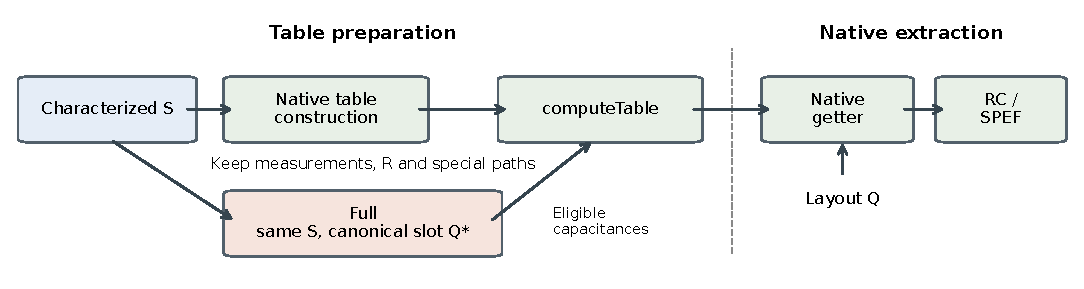
\includegraphics[width=\textwidth]{figures/compute_table_interface.pdf}
% \caption{Learning populates eligible internal capacitance slots during preparation. The original constructor supplies the complete native table; the hook changes only covered coupling/fringe values. Real observations, resistance and special returns remain native. Layout queries retain the original getter and RC assembly.}\label{fig:interface}
% \end{figure*}
% Figure~\ref{fig:interface} separates preparation from native queries. The preparation hook runs immediately after OpenRCX constructs a distance compute table and before getters use it. Keys include process/corner, rule/configuration identity, family, layers, mapped width, slot index, represented separation, output components and units. Predictions are evaluated at the coordinate represented by the slot, not at an arbitrary raw request. All S values remain real observations; generated values are never fed back as support.

% The evaluated scope is finite, non-sentinel OVER/UNDER/OVERUNDER tables with uniquely matched source-held-out rules. Measurement-bin collisions, special tails, unsupported paths and resistance remain native. Boundary paths that return the measure table are preserved. Only coupling and fringe compute fields are written. Full-grid preparation uses deterministic coordinate order and Q chunks of 32; no query-dependent Transformer support states are cached.

% We compare unmodified extraction, interface-disabled extraction, native-value pass-through, Binary and Full injection. A separate trace build checks getter values; the release build leaves getter bodies unchanged. Inventories must match across both designs of each process before claiming design-independent grid reuse. The pinned public API defers loading until extraction, so the first inventory extraction is charged to preparation. This is explicit measured overhead, not a free rule-only operation.



\section{Estimator and Compute-Table Preparation}
\subsection{Input Encoding and Contextual Representation}

Given a characterized rule, let
$\mathcal{X}=\{\mathbf{x}_i\}_{i=1}^{N}$ denote its
candidate geometry coordinates and
$\mathcal{O}\subseteq\{1,\ldots,N\}$ the observed
characterization indices. Each observation has a
$K$-dimensional capacitance vector
$\mathbf{y}_i\in\mathbb{R}^{K}$.
The remaining coordinates form the query set
$\mathcal{Q}=\{1,\ldots,N\}\setminus\mathcal{O}$.
The objective is to estimate capacitances at
unobserved geometries using only the available
characterization samples and process context.

\textbf{Input Encoding.}
We construct each geometric token from normalized
coordinates, process context, observed capacitances,
observation status, and a numerical anchor.
The normalized geometric coordinates are
\begin{equation}
\widetilde{\mathbf{x}}_i
=
\log\left(
\mathbf{1}+\mathbf{x}_i\oslash\mathbf{s}_x
\right),
\end{equation}
where $\mathbf{s}_x$ denotes the source-derived
coordinate scales. The observed capacitance vector
is encoded as
\begin{equation}
\widetilde{\mathbf{y}}_i
=
o_i(\mathbf{y}_i\oslash\mathbf{s}_y),
\qquad
o_i=\mathbb{1}[i\in\mathcal{O}],
\end{equation}
where $\mathbf{s}_y$ contains the source-derived
capacitance scales. The indicator $o_i$ distinguishes
unobserved entries from observed zero-valued
capacitances.

Let $\mathbf{c}$ denote the process and structural
context, including pattern family, metal-layer
identity, adjacent-layer context, and material
descriptors. With the normalized numerical anchor
$\widetilde{\mathbf{b}}_i=\mathbf{b}_i\oslash\mathbf{s}_y$,
the geometric token is
\begin{equation}
\mathbf{f}_i^{\mathrm{geo}}
=
[
\widetilde{\mathbf{x}}_i;
\mathbf{c};
\widetilde{\mathbf{y}}_i;
o_i;
\widetilde{\mathbf{b}}_i;
\mathbf{t}_{\mathrm{geo}}
],
\label{eq:input_token}
\end{equation}
where $\mathbf{t}_{\mathrm{geo}}=[1,0]$ identifies
a geometric token. Material tokens encoding layer
boundaries and relative permittivity are appended
when available, with $\mathbf{t}_{\mathrm{mat}}=[0,1]$.
Their observation and anchor channels are zero-filled.

\textbf{Contextual Representation.}
The concatenated token sequence
$\mathbf{F}$ is projected into a $d$-dimensional
embedding and processed by a Transformer encoder:
\begin{equation}
\mathbf{H}^{(0)}
=
\mathbf{F}\mathbf{W}_{\mathrm{in}}+\mathbf{b}_{\mathrm{in}},
\qquad
\mathbf{H}^{(L)}
=
\operatorname{Transformer}_{\theta}
(\mathbf{H}^{(0)},\mathbf{M}_{\mathrm{pad}}),
\label{eq:context_encoder}
\end{equation}
where $\mathbf{M}_{\mathrm{pad}}$ masks padded tokens.
We use $L=2$ layers, four attention heads, and
$d=64$ hidden dimensions. The contextual
representation of query $i$ is
\begin{equation}
\mathbf{h}_i=\mathbf{H}^{(L)}_i
\in\mathbb{R}^{d}.
\label{eq:context_embedding}
\end{equation}
The resulting representation captures the
relationships among observed geometries, queries,
and material context, and is shared by the residual
prediction and gating modules.


\subsection{Observation-Conditioned Residual Gating}

The estimator combines a numerical anchor with
classical and learned correction candidates.
A component-wise gating network determines their
contributions according to the contextual
representation, support geometry, and candidate
agreement.

\textbf{Numerical Anchor and Correction Basis.}
For query $\mathbf{x}_i$, let $b_{i,k}$ denote the
numerical anchor for capacitance component $k$.
It is obtained through piecewise-linear interpolation
for rank-one support, simplex interpolation within
higher-rank support, and nearest-observation fallback
outside the higher-rank interpolation hull or under
degenerate configurations.

We construct a correction dictionary
\begin{equation}
\mathcal{E}=
\{
\mathrm{Anchor},
\mathrm{PCHIP},
\mathrm{WidthLinear},
\mathrm{GP}_{\ell,\lambda},
\mathrm{NN},
\mathrm{NN\text{-}Clip}
\},
\label{eq:correction_basis}
\end{equation}
where $\ell\in\{0.5,1,2\}$ and
$\lambda\in\{10^{-6},10^{-4}\}$ define six
RBF-GP configurations. PCHIP and width-aligned
interpolation are activated only when their
support requirements are satisfied.

Each applicable candidate is represented by its
correction relative to the common anchor:
\begin{equation}
\Delta_{i,e,k}=f_{i,e,k}-b_{i,k},
\qquad
\Delta_{i,\mathrm{Anchor},k}=0,
\label{eq:correction}
\end{equation}
where $f_{i,e,k}$ denotes the candidate prediction.
A validity indicator $m_{i,e}\in\{0,1\}$ identifies
whether candidate $e$ is applicable to query $i$.
The complete dictionary contains eleven candidate
branches, including the anchor and two neural
corrections.

\textbf{Neural Residual and Agreement-aware Gating.}
The Transformer representation is mapped to a
neural residual through a linear prediction head:
\begin{equation}
\Delta_{i,\mathrm{NN},k}
=
\mathbf{w}_k^{\mathsf T}\mathbf{h}_i
+b_k^{\mathrm{NN}}.
\label{eq:neural_residual}
\end{equation}
An additional envelope-clipped residual is defined as
\begin{equation}
\Delta_{i,\mathrm{NN\text{-}Clip},k}
=
\begin{cases}
\operatorname{clip}
(b_{i,k}+\Delta_{i,\mathrm{NN},k},
L_{i,k},U_{i,k})-b_{i,k},
& \mathbf{x}_i\in\Omega,\\
\Delta_{i,\mathrm{NN},k},
& \mathbf{x}_i\notin\Omega,
\end{cases}
\label{eq:clipped_residual}
\end{equation}
where $\Omega$ denotes the characterized support
hull and $L_{i,k},U_{i,k}$ are the corresponding
component-wise envelope bounds.

To characterize candidate agreement, we calculate
the mean, standard deviation, and range of valid
corrections:
\begin{align}
\mu_{i,k}
&=
\frac{1}{N_i}
\sum_{e\in\mathcal{E}}
m_{i,e}\Delta_{i,e,k},\\
\sigma_{i,k}
&=
\sqrt{
\frac{1}{N_i}
\sum_{e\in\mathcal{E}}
m_{i,e}(\Delta_{i,e,k}-\mu_{i,k})^2
+\epsilon
},\\
r_{i,k}
&=
\max_{e:m_{i,e}=1}\Delta_{i,e,k}
-
\min_{e:m_{i,e}=1}\Delta_{i,e,k},
\end{align}
where $N_i=\sum_{e\in\mathcal{E}}m_{i,e}$ and
$\epsilon=10^{-12}$. The gating input combines
these statistics with the contextual representation
and label-blind support descriptors:
\begin{equation}
\mathbf{v}_i=
[
\mathbf{h}_i;
\mathbf{u}_i;
\phi(\boldsymbol{\mu}_i);
\phi(\boldsymbol{\sigma}_i);
\phi(\mathbf{r}_i)
],
\qquad
\phi(z)=\operatorname{sign}(z)\log(1+|z|),
\label{eq:gating_input}
\end{equation}
where $\mathbf{u}_i$ contains support density,
nearest-observation distance, local span,
hull membership, support-region indicators,
affine rank, width validity, coordinate coverage,
and local variation, slope, and curvature features.

A two-layer MLP generates candidate-specific
logits with a hidden dimension of 32:
\begin{equation}
\mathbf{a}_i
=
\mathbf{W}_{g,2}
\operatorname{ReLU}
(\mathbf{W}_{g,1}\mathbf{v}_i+\mathbf{b}_{g,1})
+\mathbf{b}_{g,2}.
\label{eq:gating_logits}
\end{equation}
The logits are combined with learnable candidate
priors $\beta_e$ and a learnable temperature
$\tau=\operatorname{softplus}(\theta_\tau)+10^{-3}$.
The component-wise gating weights are obtained by
a validity-masked softmax:
\begin{equation}
\pi_{i,e,k}
=
\frac{
m_{i,e}\exp((a_{i,e,k}+\beta_e)/\tau)
}{
\sum_{j\in\mathcal{E}}
m_{i,j}\exp((a_{i,j,k}+\beta_j)/\tau)
}.
\label{eq:gating_weights}
\end{equation}
The anchor and neural branches are initialized
without prior suppression, whereas classical
non-anchor corrections start with a negative
logit offset.

\textbf{Residual Fusion.}
The final capacitance estimate is obtained by
fusing the anchor with the weighted corrections:
\begin{equation}
\widetilde{y}_{i,k}
=
b_{i,k}
+
\sum_{e\in\mathcal{E}}
\pi_{i,e,k}\Delta_{i,e,k}.
\end{equation}
To enforce non-negative capacitance, the output
is projected onto the non-negative domain:
\begin{equation}
\widehat{y}_{i,k}
=
\left[
b_{i,k}
+
\sum_{e\in\mathcal{E}}
\pi_{i,e,k}\Delta_{i,e,k}
\right]_{+},
\qquad
[z]_{+}=\max(0,z).
\label{eq:final_prediction}
\end{equation}
All predictions are represented in source-normalized
units and are converted back to physical units
using $\mathbf{s}_y$.

Ungated uses $[b+r_{\rm NN}]_+$ and Binary uses
$[b+\alpha r_{\rm NN}]_+$ with component-wise $0\leq\alpha\leq1$.
Binary retains support descriptors but removes numerical corrections,
NN-Clip, and agreement features. These separately trained models have their
own neural parameters, so their differences do not isolate a single gate
coefficient. Full's weights normalize over valid candidates, but candidate
validity is not accuracy; agreement is neither calibrated uncertainty nor
a no-regression certificate.

\subsection{Native Compute-Table Population}

The estimator is integrated into the native
rule-based extraction flow by populating eligible
internal capacitance entries during preparation.
The original compute-table constructor, runtime
getters, and downstream parasitic-network assembly
are retained.

\textbf{Compute-Table Preparation.}
Let $\mathcal{T}$ denote the native distance
compute table constructed for rule descriptor
$\mathcal{R}$. Each table slot $j$ is associated
with a represented geometry coordinate
$\mathbf{q}_j$ and a composite key containing
process/corner, rule identity, pattern family,
routing layers, mapped width, slot index,
separation, output components, and units.

The eligible slot set is
\begin{equation}
\mathcal{J}
=
\left\{
j\in\mathcal{T}:
\begin{array}{l}
j\text{ is finite and non-sentinel},\\
j\text{ has a unique source-rule match},\\
j\text{ belongs to an eligible pattern family}
\end{array}
\right\},
\label{eq:eligible_slots}
\end{equation}
where the eligible families are OVER, UNDER,
and OVERUNDER. Rule matching uses source, family, layer context, corner,
and ordered geometry; hidden capacitances never determine eligibility. Measurement-bin collisions,
special tails, unsupported paths, and resistance
entries are excluded. Supplied measurement values
and native measure-table return paths remain
unchanged.

Predictions are evaluated at the coordinates
represented by the eligible slots, rather than
at arbitrary runtime requests. The available characterization support $S$ is retained throughout
preparation; generated values are never reused as observations.
For sparse-native evaluation, hidden rows are physically removed before
the native constructor runs. The original full-support experiment is
reported separately. Native-sparse and all three injection arms share
the same sparse rules and resulting canonical grid; unsupported rules
remain identical across arms. Hidden capacitances therefore cannot return
through the native getter or its boundary fallback.

\textbf{Population and Native Evaluation.}
Algorithm~\ref{alg:compute_table_population} summarizes
the preparation procedure. The eligible slots
are processed in deterministic coordinate order
using query chunks of 32. Only coupling and
fringe capacitance fields are updated. Resistance,
original characterization entries, and special
returns remain native.

\begin{algorithm}[t]
\caption{Native Compute-Table Population}
\label{alg:compute_table_population}
\SetInd{0.35em}{0.5em}
\SetAlgoHangIndent{0.6em}
\Input{Rule $\mathcal{R}$; real samples $\mathcal{S}$; frozen members
$\{F_{\theta^{(m)}}\}_{m=1}^{3}$; scales $(\mathbf{s}_x,\mathbf{s}_y)$; native constructor $\mathcal{C}$}
\Output{Prepared native compute table $\mathcal{T}$}
$\mathcal{R}_S\leftarrow\operatorname{RetainAvailableSamples}(\mathcal{R},\mathcal{S})$\;
$\mathcal{T}\leftarrow\mathcal{C}(\mathcal{R}_S)$\;
$\mathcal{J}\leftarrow\operatorname{SortByCoordinate}(\operatorname{EligibleSlots}(\mathcal{T},\mathcal{R},\mathcal{S}))$\;
\While{$\mathcal{J}\ne\emptyset$}{
 $\mathcal{J}_b\leftarrow\operatorname{TakeNext}(\mathcal{J},32)$\;
 $\mathcal{Q}_b\leftarrow(\mathbf{q}_j)_{j\in\mathcal{J}_b}$\;
 $(\mathbf{F}_b,\mathcal{D}_b,\mathcal{I}_b,\mathbf{M}_{\rm pad})\leftarrow\operatorname{Encode}(\mathcal{S},\mathcal{Q}_b,\mathcal{R},\mathbf{s}_x,\mathbf{s}_y)$\;
 \ForEach{frozen member $m=1,2,3$ (eval mode)}{
  $\mathbf{H}_b\leftarrow\operatorname{Transformer}_{\theta^{(m)}}(\mathbf{F}_b\mathbf{W}_{\rm in}+\mathbf{b}_{\rm in},\mathbf{M}_{\rm pad})$\;
  \ForEach{$i\in\operatorname{Unique}(\mathcal{I}_b)$}{
   $\mathbf{b}_i\leftarrow\operatorname{Anchor}(\mathcal{D}_b,i)$\;
   $(\boldsymbol{\Delta}_i,\mathbf{m}_i,\mathbf{u}_i)\leftarrow\operatorname{ResidualBasis}_{\theta^{(m)}}(\mathbf{H}_b[i],\mathcal{D}_b,i)$\;
   $(\boldsymbol{\mu}_i,\boldsymbol{\sigma}_i,\mathbf{r}_i)\leftarrow\operatorname{Agreement}(\boldsymbol{\Delta}_i,\mathbf{m}_i;10^{-12})$\;
   $\mathbf{a}_i\leftarrow\operatorname{Gate}_{\theta^{(m)}}([\mathbf{H}_b[i];\mathbf{u}_i;\phi(\boldsymbol{\mu}_i);\phi(\boldsymbol{\sigma}_i);\phi(\mathbf{r}_i)])$\;
   $\boldsymbol{\pi}_i\leftarrow\operatorname{MaskedSoftmax}_e(\mathbf{a}_i+\boldsymbol{\beta},\mathbf{m}_i,\tau)$\;
   $\widehat{\mathbf{y}}_i^{(m)}\leftarrow[\mathbf{b}_i+\sum_{e\in\mathcal{E}}\boldsymbol{\pi}_{i,e}\odot\boldsymbol{\Delta}_{i,e}]_+$\;
  }
  $\widehat{\mathbf{Y}}_b^{(m)}\leftarrow\operatorname{Rescale}((\widehat{\mathbf{y}}_{i(j)}^{(m)})_{j\in\mathcal{J}_b},\mathbf{s}_y)$\;
 }
 $\widehat{\mathbf{Y}}_b\leftarrow\frac{1}{3}\sum_{m=1}^{3}\widehat{\mathbf{Y}}_b^{(m)}$\;
 $\widehat{\mathbf{Y}}_b\leftarrow\operatorname{RestoreExactObservations}(\widehat{\mathbf{Y}}_b,\mathcal{S},\mathcal{Q}_b)$\;
 $\widehat{\mathbf{Y}}_b^{\rm native}\leftarrow\operatorname{CheckedNativeValues}(\widehat{\mathbf{Y}}_b,\mathcal{R})$\;
 $\mathcal{T}_{\mathcal{J}_b}^{\rm Cc,Cf}\leftarrow\widehat{\mathbf{Y}}_b^{\rm native}[:,\mathrm{Cc,Cf}]$\;
 $\mathcal{J}\leftarrow\mathcal{J}\setminus\mathcal{J}_b$\;
}
\Return{$\mathcal{T}$}\;
\end{algorithm}

\emph{Algorithm operations.}
$\operatorname{EligibleSlots}$ applies (\ref{eq:eligible_slots}) to initialized slots within one process/corner, pattern, layer and mapped-width context, requiring at least four original candidate samples, using the available capped budget, no sentinel tail or measurement-bin conflict, and native interior-bin eligibility. Sorting uses represented separation and then full slot key; $\mathbf{q}_j$ is the slot geometry in model units. $\operatorname{Encode}$ orders unique support tokens before query tokens, appends material tokens, caches scaled support state $\mathcal{D}_b$, and maps slots to query indices $i(j)$ through $\mathcal{I}_b$.

$\operatorname{ResidualBasis}$ assembles Anchor, PCHIP, WidthLinear, six RBF-GPs, NN and NN-Clip. Anchor has zero correction and is always valid; PCHIP requires single-width support, and WidthLinear requires aligned brackets or an exact hit. Nonfinite numerical predictions are masked. NN uses the residual head; NN-Clip clips the completed value to the support envelope only inside the observed affine space and hull, then subtracts the anchor. Both neural masks are valid; nonfinite corrections become zero.

$\operatorname{Agreement}$ computes valid-only component-wise mean, standard deviation and range. $\operatorname{Gate}$ implements (\ref{eq:gating_input})--(\ref{eq:gating_logits}); masked softmax sets invalid logits to $-10^9$ before division by $\tau=\operatorname{softplus}(\theta_\tau)+10^{-3}$. All parameters, including priors and temperature, belong to the current frozen member. $\operatorname{CheckedNativeValues}$ converts units and validates finite, nonnegative predictions before writing only eligible coupling/fringe fields. Observations, resistance, special tails and native return paths remain unchanged; $\mathcal{S}$ never includes predictions.

\begin{figure*}[t]
\centering
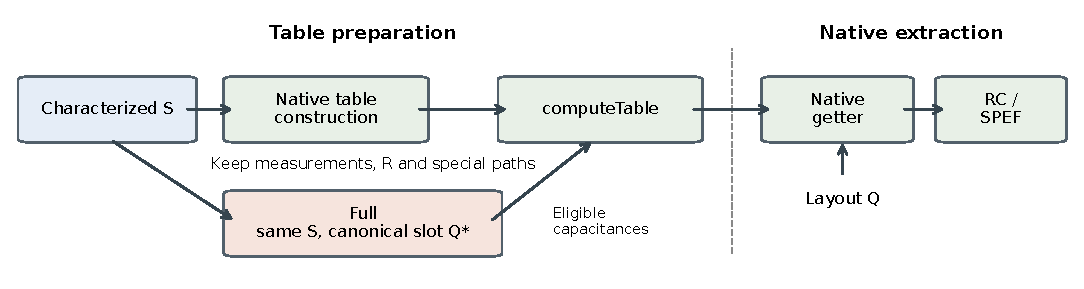
\includegraphics[width=\textwidth]
{figures/compute_table_interface.pdf}
\caption{Native compute-table population interface.
The original constructor receives the available samples $S$
(hidden rows are removed in the sparse protocol) and generates the native
evaluation structure, after which the preparation
hook selectively updates eligible coupling and
fringe capacitance entries. Supplied measurements,
resistance entries, and special return paths are
preserved. Runtime layout queries continue to use
the original getters and parasitic-network assembly.}
\label{fig:interface}
\end{figure*}



The prepared table is subsequently consumed by
the unchanged native getters, which retain
width selection, coordinate mapping, and
compute-grid quantization. Resistance evaluation
and RC-network assembly are unaffected.
We evaluate unmodified extraction, interface-disabled
extraction, native-value pass-through, Full
injection, and Binary injection as an ablation control. A separate trace
build verifies getter values, while the release
build leaves the original getter implementations
unchanged.

The pinned public API defers table loading until
extraction. Therefore, the first inventory
extraction is included in the preparation cost,
rather than treated as a free rule-only operation.
Preparation and native extraction costs are
measured and reported separately.


\section{Experimental Setup}
\subsection{Data and training}
Table~\ref{tab:data} summarizes the datasets and source-training budgets. FEM data cover FreePDK15 and ASAP7; cross-process prediction trains and selects on FreePDK15 and evaluates on ASAP7. The 84 native holdout tables are excluded from source fitting and selection. Learned completion predictions average three trained members.
The raw public inventory has 1,713 tables. Reserving 84 native holdouts
leaves 1,061 fitting and 247 selection tables, reduced by exact-curve
deduplication to 1,051 and 246. The retrospective confirmation cohort
retains the original 341 test tables (340 unique curves, 338 budget-eligible),
including 20 tables later reserved for native evaluation. These protocols
therefore do not provide independent confirmation populations. Confirmation scores reused for the present
default-selection and mechanism analysis are post-hoc evidence.

Full/Binary/Ungated optimize source-scaled component Huber loss
($\delta=1$), with one sampled episode per family per update, uniform
family weights, AdamW learning rate $2\times10^{-4}$ and weight decay
$10^{-4}$. The frozen recipe uses gradient clipping at 1, no dropout,
two Transformer layers of width 64, four heads, and gate hidden width 32.
Source residual initialization and source-fitted scales are reused;
the residual initializer itself has 2k source-only updates in each domain,
in addition to the reported 24k/12k fusion stages. The final prescribed
step is retained. MLP/CNP use 3k updates, three
members and source selection over learning rates $10^{-3}$ and
$3\times10^{-4}$; MLP adaptation is selected from 0/50/200 steps.
Adapted AttentionCap uses 3k updates with batches of up to 32 geometries,
three members and the same learning-rate/adaptation grid. Its supervision
is the three task components, not complete capacitance matrices. These
are documented, unequal training opportunities; identical $B$ matches
target observations, not total source training or tuning cost.

Three bounded controls test the fusion mechanism. C1 learns a numerical-only
gate over Anchor, PCHIP, WidthLinear, and six GPs, retaining numerical/support
features and agreement but removing the Transformer state, NN, and NN-Clip.
C3 retains Full's other inputs and candidates and is retrained without
agreement features. Both use three members, the original source pools,
sampler, optimizer, and 24k/12k final-stage budgets, without a new tuning grid.
C1 retains the source scales and gate priors but has no pretrained neural
trunk to initialize after that trunk is removed.
C2 instead freezes each Full member's candidate outputs and fits fixed
nonnegative component-wise weights on source fitting data, renormalized
over valid candidates at inference. A single frozen recipe uses three
30\%-holdout protocols per source table, seed 11, family/table-balanced
Huber loss, and 300 Adam steps at 0.05; source selection is evaluated before
confirmation. C2 is a post-hoc intervention on learned candidates, not a
retrained fixed-fusion architecture or an exhaustive search over mixtures.

\begin{table}[t]
\centering
\caption{Data and source-training opportunities. Counts are fitting/selection/confirmation tables. Public inventory size is 1,713; k denotes 1,000 updates. Matched updates apply to Full and its Binary/Ungated ablations.}
\label{tab:data}
\footnotesize\setlength{\tabcolsep}{2.5pt}
\begin{tabular}{lccc}\toprule
 & Public & FEM & Transfer\\\midrule
Geometry rank & 1 & 2 & 2\\
Components & coupling, ground & \multicolumn{2}{c}{lateral, ground, diagonal}\\
Units & native/length & F/m & F/m\\
Fit/select/confirm & 1051/246/340 & 16/24/16 & 8/12/8\\
Fit/confirm nodes & variable & 153/128 & 153/128\\
Budgeted tables & 338 & 16 & 8\\
Matched updates & 24k & 12k & 12k\\
MLP/CNP updates & 3k & 3k & 3k\\
Adapted AC updates & -- & 3k & 3k\\\bottomrule
\end{tabular}
\end{table}

\subsection{Evaluation protocols and baselines}
Coverage sensitivity uses random, block, and boundary masks at 10/30/50/70\% holdout with seeds 11/29/47/71/101 and shared support/query sets across methods. The fixed-query budget study uses $B=4,8$ for public tables and $B=4,8,16,32,64$ for FEM and transfer.

The primary baselines are the OpenRCX kernel and specified MLI; MLI-ext. adds support-only sparse completion. Numerical controls include Anchor, source-validation-selected GP, affine interpolation, PCHIP, and IDW. Full is the proposed method; Binary and Ungated are matched ablation controls. Binary retains only anchor/neural fusion, whereas Ungated adds the neural residual to the anchor without gating. The ablations share Full's source-training pools, update budgets, and ensemble size. MLP and adapted AttentionCap~\cite{attentioncode} use 200 and 50 support-fitting steps, respectively, selected on source validation; CNP conditions directly on support. AttentionCap retains its Transformer/symmetric head and supervises the same three capacitance components.

Independent FEM evaluation uses 71 layout-parameterized templates from six ASAP7 M4/M5 contexts, with 153 characterization samples per context. Logged widths and spacings define symmetric equal-width side conductors, finite grounded planes, and an exterior grounded boundary. Support and query geometries share materials and boundary conditions; Maxwell matrices provide ground and summed lateral capacitance in F/m.

Native extraction uses AES and Ibex on ASAP7, GF180, IHP SG13G2, and Sky130HS with OpenROAD \texttt{0b54bb3203} and fixed layouts, libraries, and constraints. The archived compute-table study uses full characterization. The new
sparse-native study instead constructs each affected rule from the same
$B=4/8$ farthest-point support (seeds 11/29/47) before any injection.
Its four arms are Native-sparse, MLI-ext.-native, Binary-native, and
Full-native. Geometry-only matching identifies 72 finite held-out rules
(38/7/17/10 across ASAP7/GF180/IHP/Sky130HS); 12 short, diagonal or
special rules remain unchanged in every arm. Constant resistance in
participating rules permits row removal without changing resistance.
This caps capacitance observations per affected rule, not the entire
library characterization cost. Sparse support determines the common
canonical grid and native fallback; all original hidden rows are removed.
Rule-export fidelity compares MLI-ext., the OpenRCX kernel, and Full at $B=4/8$ with shared farthest-point support and seeds 11/29/47; budgets are capped by available candidates. The 83 eligible held-out tables are completed, with other tables retained. Rule-export timing uses $B=8$ and seed 11. Full-rule extraction supplies the reference for net-capacitance and timing fidelity.

\subsection{Metrics}
For component group $g$, normalized error is
\begin{equation}
E_g=\sqrt{\frac{\sum_{i\in Q_g}(\widehat y_i-y_i)^2}{\sum_{i\in Q_g}y_i^2}}.
\end{equation}
Groups with nonzero reference energy enter the macro-average. Coverage scores average process/family/component groups and then masks;
paired uncertainty resamples public split groups or FEM/transfer
process--layer groups, keeping correlated queries and masks together.
The 60 condition counts are descriptive, not 60 independent tests.
FEM/transfer have only four/two layer groups, limiting interval interpretation; physical scores average family/component groups. Fixed-query budget scores pool data seeds before group normalization. Support-protocol scores average member-wise, group-balanced errors. Preparation and native extraction costs are timed separately.

\section{Results}
\subsection{All four characterization holdouts}
\begin{figure*}[t]
\centering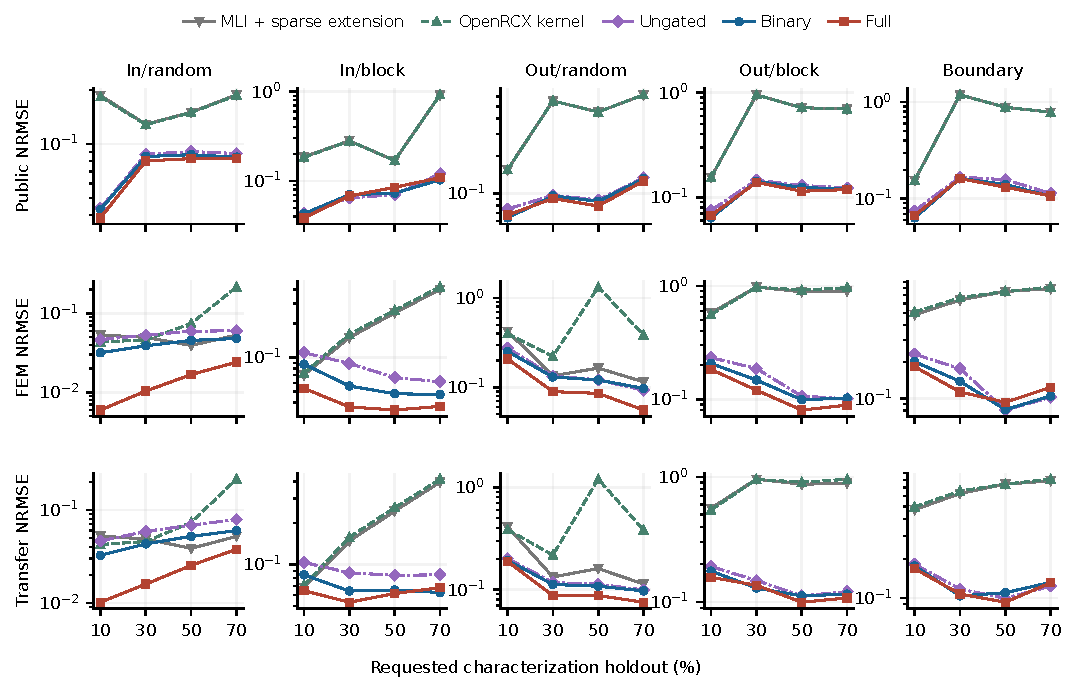
\includegraphics[width=\textwidth]{figures/coverage_four_ratios.pdf}
\caption{Coverage sensitivity: all 10/30/50/70\% holdouts, three domains and five support/protocol conditions. Mean-mask macro NRMSE on common feasible S/Q; Full and its Ungated/Binary ablations each average three matched members. MLI-ext. identifies the specified core plus declared sparse-support/boundary extension. No curve uses the native census to set holdout. Complete-cell coverage, rounded duplicates and full numerical controls are reported separately.}
\label{fig:coverage}
\end{figure*}
Figure~\ref{fig:coverage} includes all 60 domain--holdout--condition cells. Full has lower error than the OpenRCX kernel, MLI with the explicit extension, and Binary in 60, 60, and 49 cells, respectively. The kernels share 21,840/21,840 feasible support/query episodes. Complete MLI cells cover 20.7\% of requested queries across the sweep; the remainder use the declared boundary or sparse-support extension. The inventory flags 11,245 repeated rounded S/Q episodes rather than treating them as additional independent evidence. Detailed cells and all numerical controls are retained in the expanded tables.


\begin{table}[t]
\centering\small\setlength{\tabcolsep}{3pt}
\caption{Baseline-improvement consistency over all 60 conditions.
Strict wins use unrounded errors; $R=E/\min(E_{\rm ORCX},E_{\rm MLI})$
and $G=1-R$. The stronger baseline is an analysis reference, not a
deployable oracle. Float32-scale tolerance yields the same three-variant counts.}
\label{tab:consistency}
\begin{tabular}{lrrrrr}
\toprule
Method & ORCX & MLI-ext. & Both & Worst $R$ & Min. $G$ \\
\midrule
Ungated & 54/60 & 52/60 & 50/60 & 1.7780 & -77.80\% \\
Binary & 58/60 & 55/60 & 55/60 & 1.3487 & -34.87\% \\
Full & 60/60 & 60/60 & 60/60 & 0.9475 & 5.25\% \\
\bottomrule
\end{tabular}

\end{table}

Full is the only one of the three matched variants whose condition-level point estimates improve over both kernel baselines in every tested cell (Table~\ref{tab:consistency}). This motivates its unified default status, rather than requiring it to minimize every metric. Its narrowest margin is Transfer In/block at 10\% holdout: 0.064318 versus the stronger baseline 0.067879, a 5.25\% reduction. The paired error-difference interval is $[-0.01098,0.00534]$ under a 1,000-replicate layer-group bootstrap; with only two independent layer groups, this is descriptive uncertainty, not evidence that regression risk has been eliminated.

The smallest positive Ungated and Binary margins are 0.60\% and 3.01\%,
both on FEM Out/random at 30\% holdout; their paired gap intervals are
$[-0.02828,0.00923]$ and $[-0.03334,0.00552]$. Intervals overlap zero in
2/50, 4/55, and 1/60 point-improved cells for Ungated, Binary, and Full.
These correlated exploratory intervals are not independent significance
tests or a multiple-comparison guarantee.

Ungated's largest regression is Transfer In/random at 50\% holdout
(0.068591 versus 0.038578); Binary also regresses there (0.052029).
Both additionally regress on FEM and Transfer In/block at 10\% holdout.
These cases are consistent with inaccurate residual corrections when the
support-derived baseline is already accurate, but separately trained
residuals prevent a causal attribution to suppression alone. Conversely,
simple corrections can be more accurate when additional fusion is
unhelpful. All successes and regressions remain in the evaluation.

Binary is locally better than Full in 11/60 cells and Ungated in 5/60.
Binary wins include public block/interpolation and several boundary cases;
Ungated wins include public In/block at 30/50\% and FEM Boundary at
50/70\%. These outcomes are retained alongside baseline-regression cases.

At 30\% characterization holdout, Full improves over the Binary ablation in 13/15 conditions and all five FEM conditions. FEM in-support random/block errors are 0.0103/0.0366 versus Binary 0.0387/0.0560. Public Full/Binary block errors are 0.0678/0.0701, while Ungated reaches 0.0645. These observations justify component analysis rather than a universal benefit from a larger gate.

\subsection{Residual mechanisms and support conditions}
Candidate outputs, validity, member-wise weights, weighted corrections,
support counts, affine rank, and hull descriptors are recorded before an
independent scorer reads query labels. Eight illustrative conditions are
selected by a fixed post-hoc rule: each domain's smallest Full margin,
each simplified variant's worst baseline ratio, and its largest absolute
advantage over Full, merging duplicates. All 60 cells remain scored.
Diagnostic direction and SSE summaries pool query/component/member
occurrences within their stated valid sets; they are not the macro NRMSE
used for condition-level comparisons.

On Transfer In/random at 50\% holdout, the rank-two support has 64 samples.
Ungated's residual points against the required anchor correction on
19.97\% of component occurrences and exceeds twice its required magnitude
in the correct direction on 68.28\%. Binary's mean neural coefficient is
0.547; its gate reduces pooled SSE to 0.414 of its own unscaled residual
candidate, yet the final error still exceeds the stronger kernel.
Thus suppression helps that candidate without ensuring sufficient accuracy.
Full can also use different corrections: WidthLinear is valid on 59.64\%
of query occurrences and has pooled SSE 0.010 of the anchor on that subset;
the unit-length, $10^{-6}$-ridge GP has SSE 0.269 of the anchor. These
observations support complementarity as a hypothesis, rather than treating
a large gate weight as causal proof of benefit.

The narrow-margin Transfer In/block case at 10\% has 115 observations,
yet incomplete local support remains difficult. Full's GP candidates each
have larger pooled SSE than the anchor (ratios 1.26--3.36), while Full
still improves condition-level macro NRMSE. Candidate diversity alone
therefore does not explain success: conditional/component-specific fusion,
error cancellation, and different metric weighting remain possible.
Agreement is not a calibrated reliability score.

Local simplified wins show the other side. Public In/block at 50\% has
only six or seven rank-one observations: Ungated/Binary/Full errors are
0.07041/0.07307/0.08493. Full assigns mean valid weights 0.620/0.327 to
Anchor/NN-Clip and almost no weight to PCHIP, although PCHIP's pooled SSE
is 0.283 of the anchor. On FEM Boundary at 70\%, Ungated's correction
has the wrong direction on only 1.68\% of occurrences and its error
0.10271 is below Full's 0.12387. These results are consistent with useful
simple corrections being diluted, but separately trained residuals and
observational weights do not identify that as the sole cause.

\begin{table}[t]
\centering\footnotesize\setlength{\tabcolsep}{3pt}
\caption{Completed bounded controls, same 60 conditions and original
mean-mask macro errors. $^*$Both shows strict/tolerance win counts, each
out of 60. Worst $R$ uses the stronger kernel; mean $E$ is the unweighted
mean of the 60 cell errors. C2 uses frozen candidates; C1/C3 are retrained.}
\label{tab:mechanism_controls}\begin{tabular}{lrrrr}
\toprule
Method & Both$^*$ & Worst $R$ & Mean $E$ & Beats Full \\
\midrule
Full & 60/60 & 0.9475 & 0.0879 & -- \\
C2: fixed fusion & 51/51 & 12.4429 & 0.4285 & 1/60 \\
C1: numerical gate & 29/23 & 6.2401 & 0.5187 & 8/60 \\
C3: no agreement & 59/59 & 1.0359 & 0.0902 & 26/60 \\
\bottomrule
\end{tabular}

\end{table}
Table~\ref{tab:mechanism_controls} reports all 60 conditions. Numerical-only gating (C1) improves over both kernels in 29/60 cells under strict comparison (23/60 with the same numerical tolerance), with worst ratio 6.2401; it is locally better than Full in 8/60. This supports the combined neural representation/candidate pathway under this recipe, while preserving numerical-only local wins. C1 removes the Transformer state and both neural candidates together, so it does not isolate each element. The frozen-candidate fixed mixture (C2) improves both kernels in 51/60 cells and has worst ratio 12.4429, versus Full's 0.9475. This intervention supports adaptive weighting relative to the tested source-fitted mixture, not superiority over every possible fixed mixture or a retrained fixed-fusion architecture.

Removing agreement with matched retraining (C3) yields 59/60 strict improvements (59/60 with tolerance), worst ratio 1.0359, and 26/60 local wins over Full. The unweighted means of condition errors are 0.09022 for C3 and 0.08786 for Full. This provides conditional evidence for agreement in this training recipe, without establishing its necessity in other settings. These source-trained interventions remain post-hoc analyses of correlated confirmation conditions, not independent evidence of a safety guarantee.


\begin{table*}[t]
\centering\footnotesize\setlength{\tabcolsep}{5pt}
\caption{MLI status and support-region diagnostics. Queries count repeated
mask occurrences; errors average the available condition-level mean-mask
macro NRMSE within each stratum. Different strata have different coverage
and these means do not recombine by simple query-count weighting.}
\label{tab:mli_strata}\begin{tabular}{lllrrrrr}
\toprule
Domain & Status & Region & Queries & MLI & Ungated & Binary & Full \\
\midrule
Public & Complete cell & inside & 32482 & 0.2764 & 0.0761 & 0.0735 & 0.0731 \\
Public & Clamp & outside & 65033 & 0.6095 & 0.1151 & 0.1083 & 0.1059 \\
FEM & Complete cell & inside & 1920 & 0.0884 & 0.0872 & 0.0687 & 0.0371 \\
FEM & Clamp & outside & 11280 & 0.6561 & 0.1628 & 0.1445 & 0.1489 \\
FEM & Sparse extension & inside & 25424 & 0.1367 & 0.0678 & 0.0498 & 0.0275 \\
FEM & Sparse extension & outside & 10576 & 0.5508 & 0.1594 & 0.1452 & 0.1194 \\
Transfer & Complete cell & inside & 960 & 0.0856 & 0.0951 & 0.0762 & 0.0551 \\
Transfer & Clamp & outside & 5640 & 0.6454 & 0.1410 & 0.1376 & 0.1359 \\
Transfer & Sparse extension & inside & 12712 & 0.1345 & 0.0756 & 0.0575 & 0.0421 \\
Transfer & Sparse extension & outside & 5288 & 0.5412 & 0.1376 & 0.1310 & 0.1209 \\
\bottomrule
\end{tabular}

\end{table*}
Table~\ref{tab:mli_strata} separates complete cells, sparse extensions,
and clamped boundaries. Direct status replay classifies 35,362 of 171,315
query occurrences as complete cells (20.64\%). The archived 20.71\%
count included 120 singleton-support requests from two all-zero two-node
tables; their query lies outside the constant support and is now explicitly
classified as clamped. Returned values and all aggregate MLI errors are
unchanged. Full improves over MLI in all eight Public complete-cell
conditions, but only three of four FEM and two of four Transfer complete-cell
conditions. Most exposure uses sparse extension or boundary handling, so
the overall result cannot be attributed solely to multilinear interpolation's
complete-cell core.

\subsection{Task-specific interpolation under fixed budgets}
\begin{table*}[t]
\centering\footnotesize\setlength{\tabcolsep}{4pt}
\caption{Retained numerical controls at 30\% holdout, reaggregated from
their original records. Mean-mask macro NRMSE; the source-selected affine
control and fixed RBF-GP/PCHIP/IDW recipes retain their original definitions.
These are separate numerical methods, not an oracle chosen using target errors.}
\label{tab:numerical_thirty}\begin{tabular}{llrrrrrrrr}
\toprule
Domain & Queries & Anchor & Affine & RBF-GP & PCHIP & IDW & Ungated & Binary & Full \\
\midrule
Public & In/random & 0.1286 & 0.2062 & 0.4011 & 0.1070 & 0.1911 & 0.0875 & 0.0850 & 0.0803 \\
Public & In/block & 0.2812 & 0.4324 & 0.2490 & 0.1891 & 0.2733 & 0.0645 & 0.0701 & 0.0678 \\
Public & Out/random & 0.5531 & 0.4766 & 0.9120 & 0.5531 & 0.6235 & 0.0965 & 0.0954 & 0.0910 \\
Public & Out/block & 0.9546 & 0.5588 & 3.5596 & 0.9546 & 1.5155 & 0.1455 & 0.1420 & 0.1391 \\
Public & Boundary & 1.1867 & 0.6503 & 4.6800 & 1.1867 & 1.9906 & 0.1675 & 0.1629 & 0.1620 \\
FEM & In/random & 0.0208 & 0.0389 & 0.0116 & 0.0389 & 0.1337 & 0.0529 & 0.0387 & 0.0103 \\
FEM & In/block & 0.1286 & 0.1579 & 2.8414 & 0.0997 & 0.9631 & 0.0885 & 0.0560 & 0.0366 \\
FEM & Out/random & 0.0606 & 0.0621 & 1.0237 & 0.2220 & 3.7321 & 0.1336 & 0.1303 & 0.0895 \\
FEM & Out/block & 0.6542 & 0.3374 & 18.3431 & 0.9767 & 5.2144 & 0.1867 & 0.1479 & 0.1203 \\
FEM & Boundary & 0.5663 & 0.2376 & 17.6758 & 0.6691 & 3.8558 & 0.1761 & 0.1388 & 0.1137 \\
Transfer & In/random & 0.0205 & 0.0381 & 0.0113 & 0.0384 & 0.1331 & 0.0588 & 0.0432 & 0.0159 \\
Transfer & In/block & 0.1246 & 0.1542 & 2.5309 & 0.0974 & 0.9024 & 0.0868 & 0.0640 & 0.0531 \\
Transfer & Out/random & 0.0595 & 0.0594 & 0.8194 & 0.2173 & 3.1647 & 0.1172 & 0.1124 & 0.0877 \\
Transfer & Out/block & 0.6374 & 0.3288 & 16.0145 & 0.9562 & 4.7812 & 0.1482 & 0.1291 & 0.1358 \\
Transfer & Boundary & 0.5580 & 0.2364 & 15.5718 & 0.6574 & 3.5543 & 0.1172 & 0.1037 & 0.1073 \\
\bottomrule
\end{tabular}

\end{table*}
Field-solver surrogates learn geometry-to-capacitance mappings, whereas rule interpolation must use the characterized response of the current process. We evaluate this distinction with identical observed geometries and sealed queries, pooling three data seeds before group normalization. Full keeps its learned parameters fixed; adapted AttentionCap retains its geometry/material Transformer and symmetric head and fits the target capacitance components using the same support~\cite{attentioncap,attentioncode}. Figure~\ref{fig:budget_controls} reports the fixed-budget comparisons.

\begin{figure*}[t]
\centering
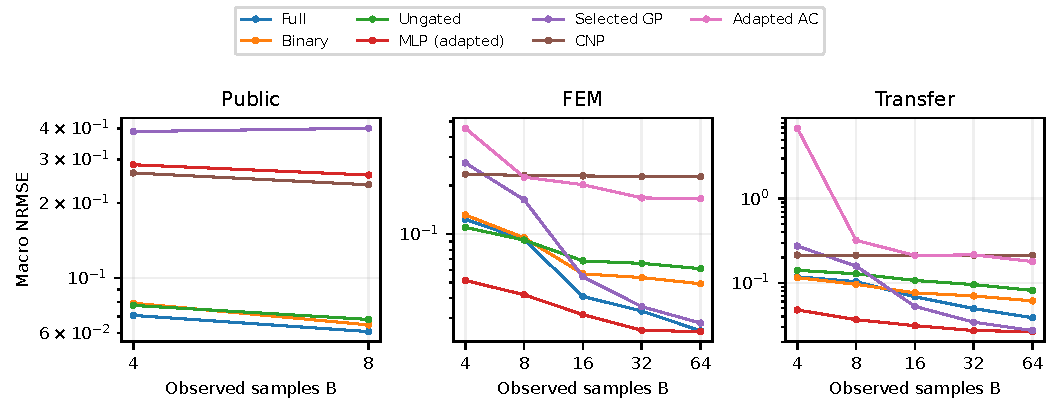
\includegraphics[width=\textwidth]{figures/fixed_budget_strong_controls.pdf}
\caption{Fixed-budget comparison including source-selected GP, target-adapted MLP, CNP, component-supervised adapted AttentionCap (AC), and all three variants. Pooled-replicate macro NRMSE (log scale; lower is better) on the same $B$ observed geometries and sealed queries. Public evaluations use $B=4/8$; adapted AC is unavailable there. Transfer targets ASAP7.}
\label{fig:budget_controls}
\end{figure*}

\begin{table*}[t]
\centering\footnotesize\setlength{\tabcolsep}{4pt}
\caption{Strong numerical and learned controls at fixed budgets; unchanged pooled-seed macro NRMSE. No target-query oracle selects among numerical methods.}\label{tab:strong}
\begin{tabular}{llrrrrrrrr}
\toprule
Domain & $B$ & Anchor & GP & PCHIP & Affine & MLP & Ungated & Binary & Full \\
\midrule
Public & 4 & 0.4229 & 0.3887 & 0.3906 & 0.4266 & 0.2860 & 0.0776 & 0.0793 & 0.0708 \\
Public & 8 & 0.3689 & 0.4013 & 0.3460 & 0.3532 & 0.2599 & 0.0682 & 0.0648 & 0.0609 \\
FEM & 4 & 0.3391 & 0.2767 & 0.3391 & 0.2602 & 0.0515 & 0.1100 & 0.1315 & 0.1233 \\
FEM & 8 & 0.2752 & 0.1633 & 0.2752 & 0.2253 & 0.0420 & 0.0917 & 0.0947 & 0.0925 \\
FEM & 16 & 0.1525 & 0.0543 & 0.1525 & 0.1709 & 0.0316 & 0.0681 & 0.0565 & 0.0409 \\
FEM & 32 & 0.0942 & 0.0354 & 0.0942 & 0.0986 & 0.0252 & 0.0657 & 0.0537 & 0.0332 \\
FEM & 64 & 0.0444 & 0.0280 & 0.0444 & 0.0615 & 0.0248 & 0.0609 & 0.0491 & 0.0250 \\
Transfer & 4 & 0.3358 & 0.2734 & 0.3358 & 0.2572 & 0.0477 & 0.1410 & 0.1153 & 0.1182 \\
Transfer & 8 & 0.2698 & 0.1584 & 0.2698 & 0.2217 & 0.0366 & 0.1282 & 0.0961 & 0.1034 \\
Transfer & 16 & 0.1500 & 0.0526 & 0.1500 & 0.1682 & 0.0310 & 0.1069 & 0.0762 & 0.0685 \\
Transfer & 32 & 0.0897 & 0.0341 & 0.0897 & 0.0969 & 0.0272 & 0.0954 & 0.0700 & 0.0495 \\
Transfer & 64 & 0.0435 & 0.0271 & 0.0435 & 0.0601 & 0.0264 & 0.0814 & 0.0611 & 0.0386 \\
\bottomrule
\end{tabular}

\end{table*}

Full outperforms CNP in all 12 available domain--budget settings and adapted AttentionCap in all ten FEM/transfer settings. On FEM, increasing $B$ from 4 to 64 reduces Full's error from 0.1233 to 0.0250, compared with 0.4546 to 0.1657 for adapted AttentionCap. On transfer, the corresponding errors are 0.1182 to 0.0386 for Full and 6.8753 to 0.1791 for adapted AttentionCap. Public Full achieves 0.0708/0.0609 at $B=4/8$, compared with CNP's 0.2650/0.2374.

These comparisons support a representation tailored to characterization-conditioned interpolation. The numerical anchor incorporates the observed target response, while residual fusion combines source-trained corrections with applicable support-derived estimates. The advantage over the adapted matrix predictor shows that geometry-to-matrix modeling does not automatically provide an accurate rule-completion model under sparse characterization. The Ungated ablation further tests the role of fusion: at $B=64$, Full reduces error from 0.0609 to 0.0250 on FEM and from 0.0814 to 0.0386 on transfer.

Target fitting and numerical interpolation remain strong alternatives in specific regimes. At FEM $B=4$, adapted MLP achieves 0.0515 versus Full's 0.1233; at transfer $B=64$, MLP/GP achieve 0.0264/0.0271 versus Full's 0.0386. The full-support physical controls likewise favor Anchor (0.00451) over direct Full (0.01675); their complete tables remain in the extended paper. Our design therefore targets conditional completion from limited characterization, with learned values prepared before native lookup. The following subsection evaluates the resulting extraction cost.

\subsection{Downstream fidelity and native extraction cost}
In the fixed-node rule-export protocol at $B=4/8$, Full reduces net-capacitance and worst-slack errors relative to each kernel in all 16 layout--budget settings (Table~\ref{tab:downstream_fidelity}). Against either baseline, TNS deviation decreases in 13 settings and remains zero for both methods in three. The two kernels use the same operators as Figure~\ref{fig:coverage}, evaluated here on one-dimensional rule tables with shared characterization support, and yield similar downstream errors.

\begin{table}[t]
\centering
\caption{Rule-export fidelity: Full error reduction (\%) relative to each kernel, shown as $B=4/8$. C: capacitance NRMSE; WS/TNS: absolute deviations from full-table extraction. Errors are averaged over seeds 11/29/47. A dash denotes zero error for both methods.}
\label{tab:downstream_fidelity}
\scriptsize\setlength{\tabcolsep}{1pt}
\begin{tabular*}{\columnwidth}{@{\extracolsep{\fill}}lrrrrrr@{}}
\toprule
& \multicolumn{3}{c}{vs. MLI-ext.} & \multicolumn{3}{c}{vs. OpenRCX kernel} \\
\cmidrule(lr){2-4}\cmidrule(l){5-7}
Layout & C & WS & TNS & C & WS & TNS \\
\midrule
ASAP7/AES & 81.2/89.1 & 89.7/88.4 & 84.1/89.5 & 81.1/89.0 & 89.6/88.4 & 84.0/89.5 \\
ASAP7/IBEX & 81.4/89.2 & 90.3/98.3 & 85.6/96.7 & 81.3/89.2 & 90.2/98.3 & 85.5/96.7 \\
GF180/AES & 84.6/78.7 & 85.0/78.5 & 84.4/78.3 & 84.6/78.7 & 85.0/78.5 & 84.4/78.3 \\
GF180/IBEX & 84.5/78.4 & 85.1/78.7 & 84.4/77.7 & 84.5/78.4 & 85.1/78.7 & 84.4/77.7 \\
IHP/AES & 91.3/87.4 & 94.5/90.1 & --/-- & 91.3/87.4 & 94.5/90.1 & --/-- \\
IHP/IBEX & 92.5/87.6 & 93.3/88.2 & 100.0/-- & 92.5/87.5 & 93.3/88.1 & 100.0/-- \\
Sky130/AES & 89.7/87.3 & 94.5/83.5 & 97.1/76.6 & 89.9/87.3 & 94.6/83.1 & 97.1/76.2 \\
Sky130/IBEX & 88.4/85.6 & 91.1/78.0 & 89.6/81.7 & 88.6/85.6 & 91.2/77.4 & 89.8/81.1 \\
\bottomrule
\end{tabular*}

\end{table}

Against MLI-ext., for GF180/IBEX at $B=8$, capacitance NRMSE decreases from 0.0161 to 0.00348, $|\Delta\mathrm{WS}|$ from 38.25 to 8.14\,ps, and $|\Delta\mathrm{TNS}|$ from 52.74 to 11.77\,ns. Figure~\ref{fig:downstream_spatial} shows both kernel comparisons across four IBEX layouts. Mean endpoint error falls by 77.8--91.1\% relative to either baseline, with improvements in all 12 process--seed pairs for each comparison.

\begin{figure}[t]
\centering
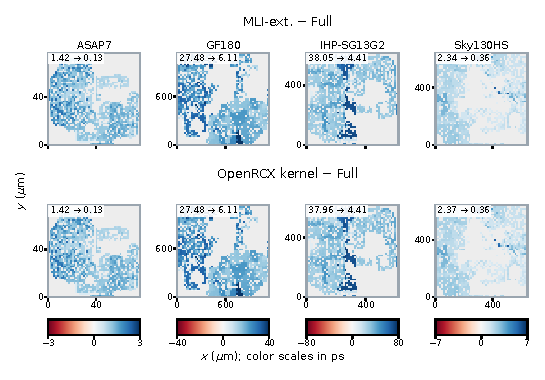
\includegraphics[width=\columnwidth]{figures/downstream_two_kernels.pdf}
\caption{Spatial timing fidelity at $B=8$, four IBEX layouts. Columns: ASAP7, GF180, IHP-SG13G2, Sky130HS. Top: MLI-ext. minus Full; bottom: OpenRCX kernel minus Full. Maps average endpoint absolute-error reductions against full-table extraction over seeds 11/29/47 and $50\times50$ bins. Annotations give baseline$\to$Full MAE (ps). Each column shares a symmetric scale: blue indicates improvement, red degradation, gray empty bins. Coordinates are in $\mu$m.}
\label{fig:downstream_spatial}
\end{figure}

\begin{table}[t]
\centering\caption{Full-characterization compute-table path, Full: full-rule net-C fidelity, mean extraction ratio over three release runs, summed external preparation stages, PEX and SPEF wall seconds. Preparation includes inventory acquisition and loading; native table build/injection remains within extraction. Output and STA costs are separately retained.}\label{tab:deployment}\small\setlength{\tabcolsep}{3pt}\begin{tabular}{lrrrrr}
\toprule
Layout & C err. & Prep. & PEX & SPEF & $T/T_0$ \\
\midrule
asap7/aes & 0.00426 & 5.41 & 2.05 & 0.49 & 0.991 \\
asap7/ibex & 0.00516 & 5.41 & 3.30 & 0.72 & 1.020 \\
gf180/aes & 0.00030 & 8.39 & 2.45 & 0.52 & 1.031 \\
gf180/ibex & 0.00020 & 8.39 & 2.73 & 0.52 & 0.999 \\
IHP/aes & 0.05656 & 13.99 & 2.00 & 0.40 & 1.035 \\
IHP/ibex & 0.05477 & 13.99 & 3.10 & 0.66 & 1.029 \\
Sky/aes & 0.00382 & 8.48 & 2.43 & 0.56 & 1.017 \\
Sky/ibex & 0.00233 & 8.48 & 2.29 & 0.58 & 1.024 \\
\bottomrule
\end{tabular}

\end{table}
The full-characterization interface populates 49,657 eligible finite slots across four rule libraries. Native-value pass-through preserves traced getter returns and electrical SPEF records on all eight layouts. Full changes 924,647 traced returns; covered returns match injected values, and resistance/uncovered returns remain identical. Table~\ref{tab:deployment} reports this archived full-characterization path: across 120 release runs, the Full extraction/original ratio ranges from 0.991 to 1.035. Summing archived inventory, input/model/support preparation and native-process startup residual, modeled first-design PEX overhead ranges from 161.1\% to 670.4\%. SPEF output and STA are measured separately and are not used to dilute this denominator. Values below one are repeat-run variation, not a stable acceleration claim.


Full's net-C fidelity error ranges from 0.00020 to 0.05656. The largest errors occur on IHP, with worst-slack changes of 74.4/147.4\,ps for AES/Ibex. These are deviations from native full-rule extraction, not improvements against an independent field reference.

The fixed-node rule-export configuration has a different support and deployment contract. Across 96 release runs, Full's extraction/original ratio is 0.983--1.047. Four-library B=8 prediction/export costs 0.70/0.67/0.91\,s for MLI-ext./Binary/Full, plus 0.88\,s shared setup; the MLI-ext. timing uses the output-equivalent archived CMI implementation. Full improves net-C and worst-slack fidelity over MLI-ext. in all 16 layout--budget cells, but improves over Binary in only six/four cells; Binary has lower P99 endpoint error in ten. These fidelity and timing results are retained without relabeling them as computeTable injection.

% Start the final discussion in the second column of the last content page.
%\newpage
\subsection{Paired sparse-native evaluation}
The sparse-native study removes the hidden rows before construction and
uses identical retained samples and native interfaces for all four arms.
Two smoke layouts cover ASAP7 and the higher-error IHP case. Poisoning
hidden labels leaves released support, sparse rules, and predictions
unchanged. Native-value pass-through, protected observation bins,
finite/nonnegative values, 1,000/2,000-DBU unit conversion, exact payload
returns, unchanged resistance and uncovered paths all pass. Every matrix
run retains the same net and endpoint identities as its full-rule reference.
These checks establish interface correctness, not physical accuracy.

The new sparse-native matrix completes all 192 arm-settings (48 paired settings, 16 layout--budget cells). Full lowers net-C, worst-slack, and P99 endpoint errors relative to Native-sparse in 7/16, 9/16, and 7/16 cells, respectively. The corresponding counts against MLI-ext.-native are 7/16, 9/16, and 7/16; against Binary-native they are 16/16, 16/16, and 16/16. These are dependent descriptive cells after averaging the three support seeds. They do not establish uniform sparse-native gains.

The mean paired Full-minus-Native-sparse differences across cells are
$+0.00509$ net-C NRMSE and $+12.40$\,ps worst-slack error. A descriptive
bootstrap that retains each process's layouts, budgets, and seeds together
gives ranges $[-0.00588,0.02157]$ and $[-6.19,44.28]$\,ps, respectively.
With only four process clusters, these are sensitivity summaries, not
reliable population confidence claims; complete paired seed ranges are retained.

\begin{figure*}[t]
\centering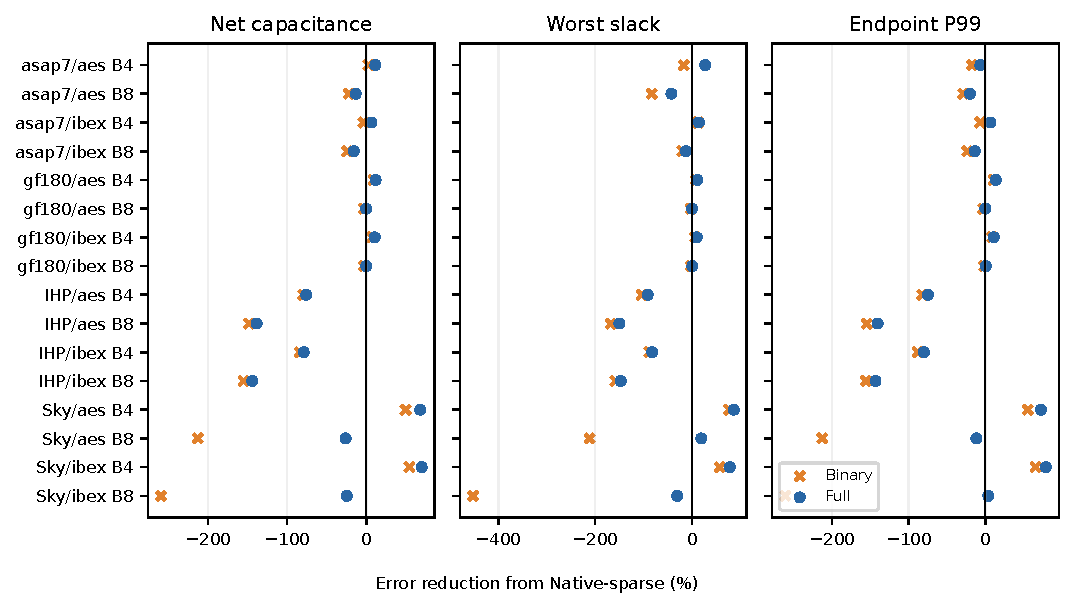
\includegraphics[width=\textwidth]{figures/native_sparse_tradeoffs.pdf}
\caption{Sparse-native Full and Binary fidelity relative to Native-sparse
across all 16 layout--budget cells. Positive values denote lower error.
Points use paired three-seed means; cells sharing a process are dependent.}
\label{fig:native_tradeoffs}
\end{figure*}

\begin{table*}[t]
\centering\footnotesize\setlength{\tabcolsep}{4pt}
\caption{Sparse-native fidelity, three-seed means. C is net-capacitance NRMSE;
WS is absolute worst-slack deviation (ps). All four arms use the same
$B$ observations per affected rule and the same sparse native table.}
\label{tab:sparse_native}\begin{tabular}{llrrrrrrrr}
\toprule
Layout & $B$ & Native C & MLI C & Binary C & Full C & Native WS & MLI WS & Binary WS & Full WS \\
\midrule
asap7/aes & 4 & 0.02486 & 0.02486 & 0.02421 & 0.02198 & 0.596 & 0.596 & 0.697 & 0.434 \\
asap7/aes & 8 & 0.02082 & 0.02082 & 0.02538 & 0.02358 & 0.360 & 0.360 & 0.659 & 0.513 \\
asap7/ibex & 4 & 0.02415 & 0.02415 & 0.02497 & 0.02253 & 4.261 & 4.261 & 3.710 & 3.667 \\
asap7/ibex & 8 & 0.02144 & 0.02144 & 0.02663 & 0.02478 & 3.868 & 3.868 & 4.630 & 4.362 \\
gf180/aes & 4 & 0.02269 & 0.02269 & 0.02057 & 0.01997 & 19.734 & 19.734 & 18.129 & 17.586 \\
gf180/aes & 8 & 0.01824 & 0.01824 & 0.01871 & 0.01824 & 15.804 & 15.804 & 16.256 & 15.798 \\
gf180/ibex & 4 & 0.01989 & 0.01989 & 0.01838 & 0.01772 & 46.683 & 46.683 & 43.624 & 42.143 \\
gf180/ibex & 8 & 0.01613 & 0.01613 & 0.01659 & 0.01613 & 38.251 & 38.251 & 39.086 & 38.032 \\
IHP/aes & 4 & 0.03266 & 0.03266 & 0.05876 & 0.05745 & 38.060 & 38.060 & 77.652 & 72.949 \\
IHP/aes & 8 & 0.02439 & 0.02439 & 0.06056 & 0.05819 & 30.442 & 30.442 & 81.560 & 76.093 \\
IHP/ibex & 4 & 0.03117 & 0.03117 & 0.05743 & 0.05580 & 82.046 & 82.046 & 154.127 & 149.496 \\
IHP/ibex & 8 & 0.02320 & 0.02320 & 0.05913 & 0.05664 & 61.411 & 61.411 & 158.647 & 151.879 \\
Sky/aes & 4 & 0.02544 & 0.02544 & 0.01278 & 0.00805 & 18.825 & 18.825 & 4.438 & 2.626 \\
Sky/aes & 8 & 0.00548 & 0.00548 & 0.01715 & 0.00690 & 2.530 & 2.530 & 7.881 & 2.051 \\
Sky/ibex & 4 & 0.02426 & 0.02426 & 0.01099 & 0.00723 & 21.908 & 21.908 & 9.413 & 4.825 \\
Sky/ibex & 8 & 0.00455 & 0.00455 & 0.01636 & 0.00566 & 2.501 & 2.501 & 13.802 & 3.265 \\
\bottomrule
\end{tabular}

\end{table*}
\begin{table*}[t]
\centering\footnotesize\setlength{\tabcolsep}{4pt}
\caption{Sparse-native endpoint P99 absolute error (ps) and absolute TNS
deviation (ns), with the same cells and seed aggregation as
Table~\ref{tab:sparse_native}.}
\label{tab:sparse_native_tails}\begin{tabular}{llrrrrrrrr}
\toprule
Layout & $B$ & Native P99 & MLI P99 & Binary P99 & Full P99 & Native TNS & MLI TNS & Binary TNS & Full TNS \\
\midrule
asap7/aes & 4 & 1.363 & 1.363 & 1.600 & 1.452 & 0.0039 & 0.0039 & 0.0047 & 0.0038 \\
asap7/aes & 8 & 1.261 & 1.261 & 1.624 & 1.513 & 0.0032 & 0.0032 & 0.0047 & 0.0042 \\
asap7/ibex & 4 & 4.460 & 4.460 & 4.752 & 4.170 & 0.0173 & 0.0173 & 0.0140 & 0.0136 \\
asap7/ibex & 8 & 4.257 & 4.257 & 5.255 & 4.842 & 0.0116 & 0.0116 & 0.0143 & 0.0133 \\
gf180/aes & 4 & 25.559 & 25.559 & 22.752 & 22.085 & 3.8625 & 3.8625 & 3.6064 & 3.4698 \\
gf180/aes & 8 & 20.094 & 20.094 & 20.617 & 20.096 & 3.1648 & 3.1648 & 3.2534 & 3.1509 \\
gf180/ibex & 4 & 62.659 & 62.659 & 57.030 & 55.743 & 65.0495 & 65.0495 & 60.3870 & 57.9268 \\
gf180/ibex & 8 & 51.014 & 51.014 & 51.819 & 50.754 & 52.7380 & 52.7380 & 54.1253 & 52.3740 \\
IHP/aes & 4 & 46.907 & 46.907 & 85.463 & 82.023 & 0.0000 & 0.0000 & 0.0000 & 0.0000 \\
IHP/aes & 8 & 34.710 & 34.710 & 88.383 & 83.457 & 0.0000 & 0.0000 & 0.0000 & 0.0000 \\
IHP/ibex & 4 & 119.879 & 119.879 & 225.798 & 215.819 & 0.0037 & 0.0037 & 0.0000 & 0.0000 \\
IHP/ibex & 8 & 90.799 & 90.799 & 232.215 & 220.752 & 0.0000 & 0.0000 & 0.0000 & 0.0000 \\
Sky/aes & 4 & 24.067 & 24.067 & 10.816 & 6.625 & 0.0777 & 0.0777 & 0.0122 & 0.0059 \\
Sky/aes & 8 & 4.884 & 4.884 & 15.261 & 5.455 & 0.0051 & 0.0051 & 0.0161 & 0.0037 \\
Sky/ibex & 4 & 48.663 & 48.663 & 16.827 & 10.296 & 5.7422 & 5.7422 & 2.4365 & 1.3615 \\
Sky/ibex & 8 & 8.053 & 8.053 & 29.069 & 7.737 & 0.6584 & 0.6584 & 3.8324 & 0.9432 \\
\bottomrule
\end{tabular}

\end{table*}
\begin{table*}[t]
\centering\footnotesize\setlength{\tabcolsep}{4pt}
\caption{Sparse-native absolute net-capacitance RMSE (fF) and Full's
relative error reduction (\%) from Native-sparse for C, WS, and P99.
Negative gains denote regression; no denominator offset is used.}
\label{tab:sparse_native_absolute}\begin{tabular}{llrrrrrrr}
\toprule
Layout & $B$ & Native C & MLI C & Binary C & Full C & C gain & WS gain & P99 gain \\
\midrule
asap7/aes & 4 & 0.031236 & 0.031236 & 0.030418 & 0.027618 & +11.6 & +27.2 & -6.5 \\
asap7/aes & 8 & 0.026155 & 0.026155 & 0.031889 & 0.029623 & -13.3 & -42.6 & -20.0 \\
asap7/ibex & 4 & 0.049514 & 0.049514 & 0.051194 & 0.046195 & +6.7 & +13.9 & +6.5 \\
asap7/ibex & 8 & 0.043951 & 0.043951 & 0.054604 & 0.050805 & -15.6 & -12.8 & -13.7 \\
gf180/aes & 4 & 0.47797 & 0.47797 & 0.43326 & 0.42081 & +12.0 & +10.9 & +13.6 \\
gf180/aes & 8 & 0.38419 & 0.38419 & 0.39407 & 0.3843 & -0.0 & +0.0 & -0.0 \\
gf180/ibex & 4 & 0.86825 & 0.86825 & 0.80232 & 0.77378 & +10.9 & +9.7 & +11.0 \\
gf180/ibex & 8 & 0.70435 & 0.70435 & 0.72413 & 0.70412 & +0.0 & +0.6 & +0.5 \\
IHP/aes & 4 & 0.41737 & 0.41737 & 0.75081 & 0.7341 & -75.9 & -91.7 & -74.9 \\
IHP/aes & 8 & 0.3116 & 0.3116 & 0.77389 & 0.74355 & -138.6 & -150.0 & -140.4 \\
IHP/ibex & 4 & 0.4518 & 0.4518 & 0.83243 & 0.80878 & -79.0 & -82.2 & -80.0 \\
IHP/ibex & 8 & 0.33633 & 0.33633 & 0.85712 & 0.82095 & -144.1 & -147.3 & -143.1 \\
Sky/aes & 4 & 0.35752 & 0.35752 & 0.17962 & 0.11317 & +68.3 & +86.0 & +72.5 \\
Sky/aes & 8 & 0.076989 & 0.076989 & 0.24111 & 0.097036 & -26.0 & +18.9 & -11.7 \\
Sky/ibex & 4 & 0.48759 & 0.48759 & 0.22096 & 0.14524 & +70.2 & +78.0 & +78.8 \\
Sky/ibex & 8 & 0.091443 & 0.091443 & 0.3288 & 0.11387 & -24.5 & -30.6 & +3.9 \\
\bottomrule
\end{tabular}

\end{table*}
\begin{table*}[t]
\centering\footnotesize\setlength{\tabcolsep}{4pt}
\caption{Separate fixed-node rule-export results: absolute net-capacitance
RMSE (fF), WS deviation (ps), and endpoint P99 error (ps). These are the
original three-seed means and are not sparse-native results.}
\label{tab:export_absolute}\begin{tabular}{llrrrrrrrrr}
\toprule
Layout & $B$ & MLI C & Binary C & Full C & MLI WS & Binary WS & Full WS & MLI P99 & Binary P99 & Full P99 \\
\midrule
asap7/aes & 4 & 0.031396 & 0.006751 & 0.0059027 & 0.5972 & 0.055419 & 0.061802 & 1.3675 & 0.36427 & 0.29751 \\
asap7/aes & 8 & 0.026218 & 0.0036477 & 0.0028695 & 0.35999 & 0.03549 & 0.041744 & 1.2737 & 0.18857 & 0.15463 \\
asap7/ibex & 4 & 0.049888 & 0.010531 & 0.0092657 & 4.3198 & 0.52425 & 0.41874 & 4.5018 & 0.89125 & 0.74405 \\
asap7/ibex & 8 & 0.043993 & 0.0060746 & 0.0047646 & 3.8691 & 0.29417 & 0.067687 & 4.2624 & 0.49659 & 0.32921 \\
gf180/aes & 4 & 0.47797 & 0.016789 & 0.073701 & 19.734 & 0.53406 & 2.9669 & 25.559 & 0.84687 & 3.9374 \\
gf180/aes & 8 & 0.38419 & 0.082205 & 0.081856 & 15.804 & 3.4111 & 3.3911 & 20.094 & 4.3845 & 4.2893 \\
gf180/ibex & 4 & 0.86825 & 0.027693 & 0.13444 & 46.683 & 1.0306 & 6.934 & 62.659 & 1.7847 & 9.4279 \\
gf180/ibex & 8 & 0.70435 & 0.15061 & 0.15204 & 38.251 & 8.1399 & 8.1449 & 51.014 & 10.918 & 10.943 \\
IHP/aes & 4 & 0.41753 & 0.027303 & 0.036225 & 38.093 & 1.7992 & 2.0818 & 46.927 & 2.4421 & 3.5196 \\
IHP/aes & 8 & 0.31155 & 0.025617 & 0.039124 & 30.439 & 1.3271 & 3.0109 & 34.7 & 2.687 & 4.056 \\
IHP/ibex & 4 & 0.45211 & 0.024323 & 0.033729 & 82.111 & 3.5604 & 5.4869 & 119.95 & 6.0355 & 8.5791 \\
IHP/ibex & 8 & 0.33629 & 0.025948 & 0.041837 & 61.402 & 4.5919 & 7.2606 & 90.781 & 6.9672 & 10.956 \\
Sky/aes & 4 & 0.35733 & 0.018492 & 0.036729 & 18.765 & 0.8488 & 1.0287 & 23.939 & 1.3221 & 2.5416 \\
Sky/aes & 8 & 0.07755 & 0.0096311 & 0.0098538 & 2.5252 & 0.42751 & 0.41559 & 4.8262 & 0.69739 & 0.71307 \\
Sky/ibex & 4 & 0.48738 & 0.028111 & 0.056394 & 21.772 & 1.2387 & 1.938 & 48.374 & 2.3872 & 4.9896 \\
Sky/ibex & 8 & 0.092147 & 0.015101 & 0.013292 & 2.4724 & 0.48909 & 0.54476 & 8.0586 & 1.2 & 1.0894 \\
\bottomrule
\end{tabular}

\end{table*}

In sparse-native IHP, Full's net-C errors are 0.05580--0.05819 versus
0.02320--0.03266 for Native-sparse; worst-slack deviations also increase.
The unit and interface checks pass, and every populated coordinate lies
within its available support's distance range; the negative fidelity results
remain despite these checks. Conversely, Sky130HS at $B=4$ shows substantially lower Full
errors. In these one-width sparse rules, MLI-ext.-native and Native-sparse
produce effectively identical downstream scores: population alone need
not change the result of linear native interpolation. The original
rule-export protocol inserts predicted characterization nodes before
construction; sparse-native instead retains the sparse constructor's grid
and fallback and fills eligible interior slots. Their different query
sets, batching, and boundary paths preclude transferring one protocol's
wins to the other. This is an interface-level explanation of the differing
contracts, not proof of a single cause for the observed gap.

\begin{table}[t]
\centering\scriptsize\setlength{\tabcolsep}{3pt}
\caption{Sparse-native costs (seconds), averaged over two budgets and
three support seeds per layout. B/F denote Binary/Full. Prep includes
shared support release, diagnostic inventory, shared model loading,
and arm-specific prediction. PEX includes native construction/injection.
$^*$Total is a sum of measured stages, including native process/SPEF/STA,
not an independently timed standalone cold launch.}
\label{tab:sparse_native_cost}\begin{tabular}{lrrrrrr}
\toprule
Layout & B prep & F prep & B PEX & F PEX & B total$^*$ & F total$^*$ \\
\midrule
asap7/aes & 11.70 & 12.11 & 2.39 & 2.48 & 21.07 & 21.44 \\
asap7/ibex & 11.70 & 12.11 & 3.95 & 3.95 & 26.34 & 26.71 \\
gf180/aes & 12.32 & 13.93 & 2.99 & 2.84 & 21.14 & 22.57 \\
gf180/ibex & 12.32 & 13.93 & 3.27 & 3.17 & 22.79 & 24.18 \\
IHP/aes & 14.29 & 18.19 & 2.50 & 2.50 & 21.62 & 25.44 \\
IHP/ibex & 14.29 & 18.19 & 3.60 & 3.53 & 24.65 & 28.52 \\
Sky/aes & 13.14 & 14.52 & 2.86 & 3.00 & 23.33 & 24.64 \\
Sky/ibex & 13.14 & 14.52 & 2.63 & 2.76 & 23.69 & 25.29 \\
\bottomrule
\end{tabular}

\end{table}
The diagnostic inventory really runs an extraction and is charged in
preparation. Its additional SPEF/STA work is retained in this conservative
cost boundary. The shared loader initializes all variant checkpoints and
is charged to each neural arm; isolated minimal per-arm cold loading was
not measured. External Python process startup/import time, source labels, exhaustive source
training/selection, and acquisition of target characterization are outside these
measured stages and are not zero-cost items.
The release runs share a host with bounded training workers, so their
single-run stage measurements do not establish a speedup. Reuse of an
unchanged support/grid/model/batching payload avoids prediction, while
each design still incurs native construction, injection, and extraction.
For an unchanged rule/support/model/query policy, the cost model is
\begin{equation}
T_{\rm total}(N)=T_{\rm reusable\ prep}+N T_{\rm native\ process}.
\end{equation}
The prepared payload was actually shared between AES and Ibex with every
eligible key applied. Larger reuse counts in Table~\ref{tab:native_reuse}
are hypothetical repetitions at the measured stage costs, not additional
timing experiments or a promise of reuse after the support or library changes.
\begin{table}[t]
\centering\small
\caption{Modeled seconds per design, $T_{\rm total}(N)/N$, averaged over the
48 settings. All columns are stage-based models, including $N=1$.
The native process includes PEX, SPEF, STA and process overhead. Native-sparse
needs no inventory/inference; its support-release cost was separately measured
with warm/uncontrolled cache. These are not equal-accuracy speedups.}
\label{tab:native_reuse}\begin{tabular}{lrrr}
\toprule
Method & $N=1$ & $N=10$ & $N=100$ \\
\midrule
Native-sparse & 10.27 & 10.17 & 10.16 \\
MLI-ext.-native & 21.11 & 11.27 & 10.28 \\
Binary-native & 23.08 & 11.50 & 10.35 \\
Full-native & 24.85 & 11.63 & 10.31 \\
\bottomrule
\end{tabular}

\end{table}

\subsection{Reused runtime and conditional limitations}
On one pinned Xeon Gold 6530 thread, three warmups and 20 interleaved blocks measure warm evaluation, with distinct Q=1/8/32 accuracy. Direct Full/Binary/Anchor at Q limit32 cost 3.706/2.110/0.788\,ms/query. Full's actual Q=1 mean is 40.97\,ms. Retained-fit MLP costs 0.025\,ms/query after 14.03\,s fitting across six contexts; adapted AttentionCap costs 0.230\,ms/query after 11.27\,s fitting, at NRMSE 0.70695. No fit uses query labels. Source training is a separate supplied-model cost; recorded final-stage times are retained in the expanded treatment, while complete source-label and training costs are unavailable.

Resident single-RHS fine FEM costs 3.719\,s/query including remeshing and factorization; 213 solves agree with certified matrix rows within $1.5\times10^{-15}$ scaled difference. Predictor errors exceed reference uncertainty, so these times do not establish an equal-accuracy speedup. The 1.72\,ns validated cache-hot getter counterpart excludes width/context resolution and assembly; it is not full PEX latency.

Global attention makes predictions depend on Q; deterministic sorting does not imply query-set invariance. With fixed support and one fixed target on one deterministically chosen long table per domain, Q=1/8/32, changed companions, and changed chunk boundaries alter predictions. The largest Full change is 0.00608 in source-normalized units; the largest across variants is 0.04600 (Ungated). Pure permutations give a smaller but nonzero maximum of $3.24\times10^{-5}$, exceeding the predeclared $8\epsilon_{32}$ scale tolerance. Duplicate queries are deduplicated and masked padding leaves outputs unchanged in these fixtures. These are limited diagnostics, not a proof of invariance or leakage. Reference-error changes and absolute units are retained with each fixture; a zero reference is never used as a relative denominator. Compute-table preparation therefore defines and scores its complete-slot batching separately from direct query replay. Support-protocol continuation can also trade sparse accuracy for retention: the matched low-budget study narrows Full's average advantage over Binary from 0.014088 to 0.002939, with denser-support degradation. The expanded treatment retains all process, budget, learning and timing controls. No query-reference-selected fallback is used.

\section{Conclusion}
We presented Full, a characterization-conditioned residual model that uses the available geometry--capacitance samples to improve rule evaluation. Its numerical anchor and gated correction basis combine the current process response with learned geometric context. The native compute-table interface prepares eligible capacitance values before lookup while preserving measured entries, resistance, and downstream extraction. Binary and Ungated serve as matched ablations that test the effects of simplifying or removing gated residual fusion.

The evaluations connect interpolation accuracy to extraction fidelity. Full lowers macro NRMSE relative to both kernel controls in all 60 coverage conditions. Separate rule-export evaluations improve capacitance and worst-slack fidelity in all 16 layout--budget settings. At $B=8$, mean endpoint slack error falls by 77.8--91.1\% across four IBEX layouts relative to either kernel. Numerical interpolation remains more accurate on the fully supported physical-reference templates, highlighting the importance of characterization coverage. Full remains the default for empirical cross-condition improvements over the two specified kernel baselines, while Binary/Ungated local optima and stronger numerical controls delimit its scope. The paired sparse-native matrix verifies label isolation and the unchanged runtime interface, but its 7/16 net-C and 9/16 worst-slack improvements over Native-sparse show that the offline result does not guarantee downstream gains. Full targets prediction under limited characterization, with learned inference performed during table preparation and native lookup retained for layout queries.
\clearpage
\bibliographystyle{IEEEtran}\bibliography{references}
\end{document}
